\clearpage
\section{Mars}
\subsection{RIMFAX}
This chapter contains published interpretations done on RIMFAX data, with the latest update of the chapter being done in May 2025. 

\begin{table}[h!]
\centering
\caption{Grouped radar interpretation keywords extracted from the RIMFAX dataset.}
\begin{tabular}{|p{6.8cm}|p{6.8cm}|}
\hline
\textbf{Geometry / Structure} & \textbf{Geometry / Structure (cont.)} \\
\hline
Bumpy & Ridge \\
Clinoform structures & Semi-horizontal layering \\
Concave up structures & Sub-horizontal \\
Crossing reflectors & Sigmoidal profiles \\
Dipping & Sloped-surface \\
Horizontal layering & Sloping reflectors \\
Hummocky & Subparallel \\
Lenticular reflectors & Transparent unit \\
Onlap & Multidirectional dipping \\
\hline
\textbf{Amplitude / Reflectivity} & \textbf{Continuity} \\
\hline
Attenuated signal & Coherent near-surface layering \\
High reflectivity & Continuous \\
Low reflectivity & Discontinuous layers \\
Strong reflectivity & Low continuity \\
Strong surface reflections & Semi-continuous \\
Weak reflectivity & Sparse internal reflections \\
Transparent zones & \\
\hline
\textbf{Terminations / Surfaces} & \textbf{Other / Descriptive} \\
\hline
Erosional contact & Chaotic \\
Truncating reflections & Parallel \\
Truncation & \\
\hline
\end{tabular}
\label{tab:rimfax-keywords}
\end{table}

\clearpage
\subsubsection{Igneous}
The article by \citet{Hamran2022} does not strictly conclude with a specific depositional environment. However, it does lean more towards an igneous explanation, thus placing the interpretations in this section. Furthermore, within the igneous hypothesis is the suggestion of the layered intrusions. There are no terrestrial GPR analogues for this structure yet, however, some of the structures within this section are interpreted as layered intrusions. 
\begin{figure}[h!]
    \centering
    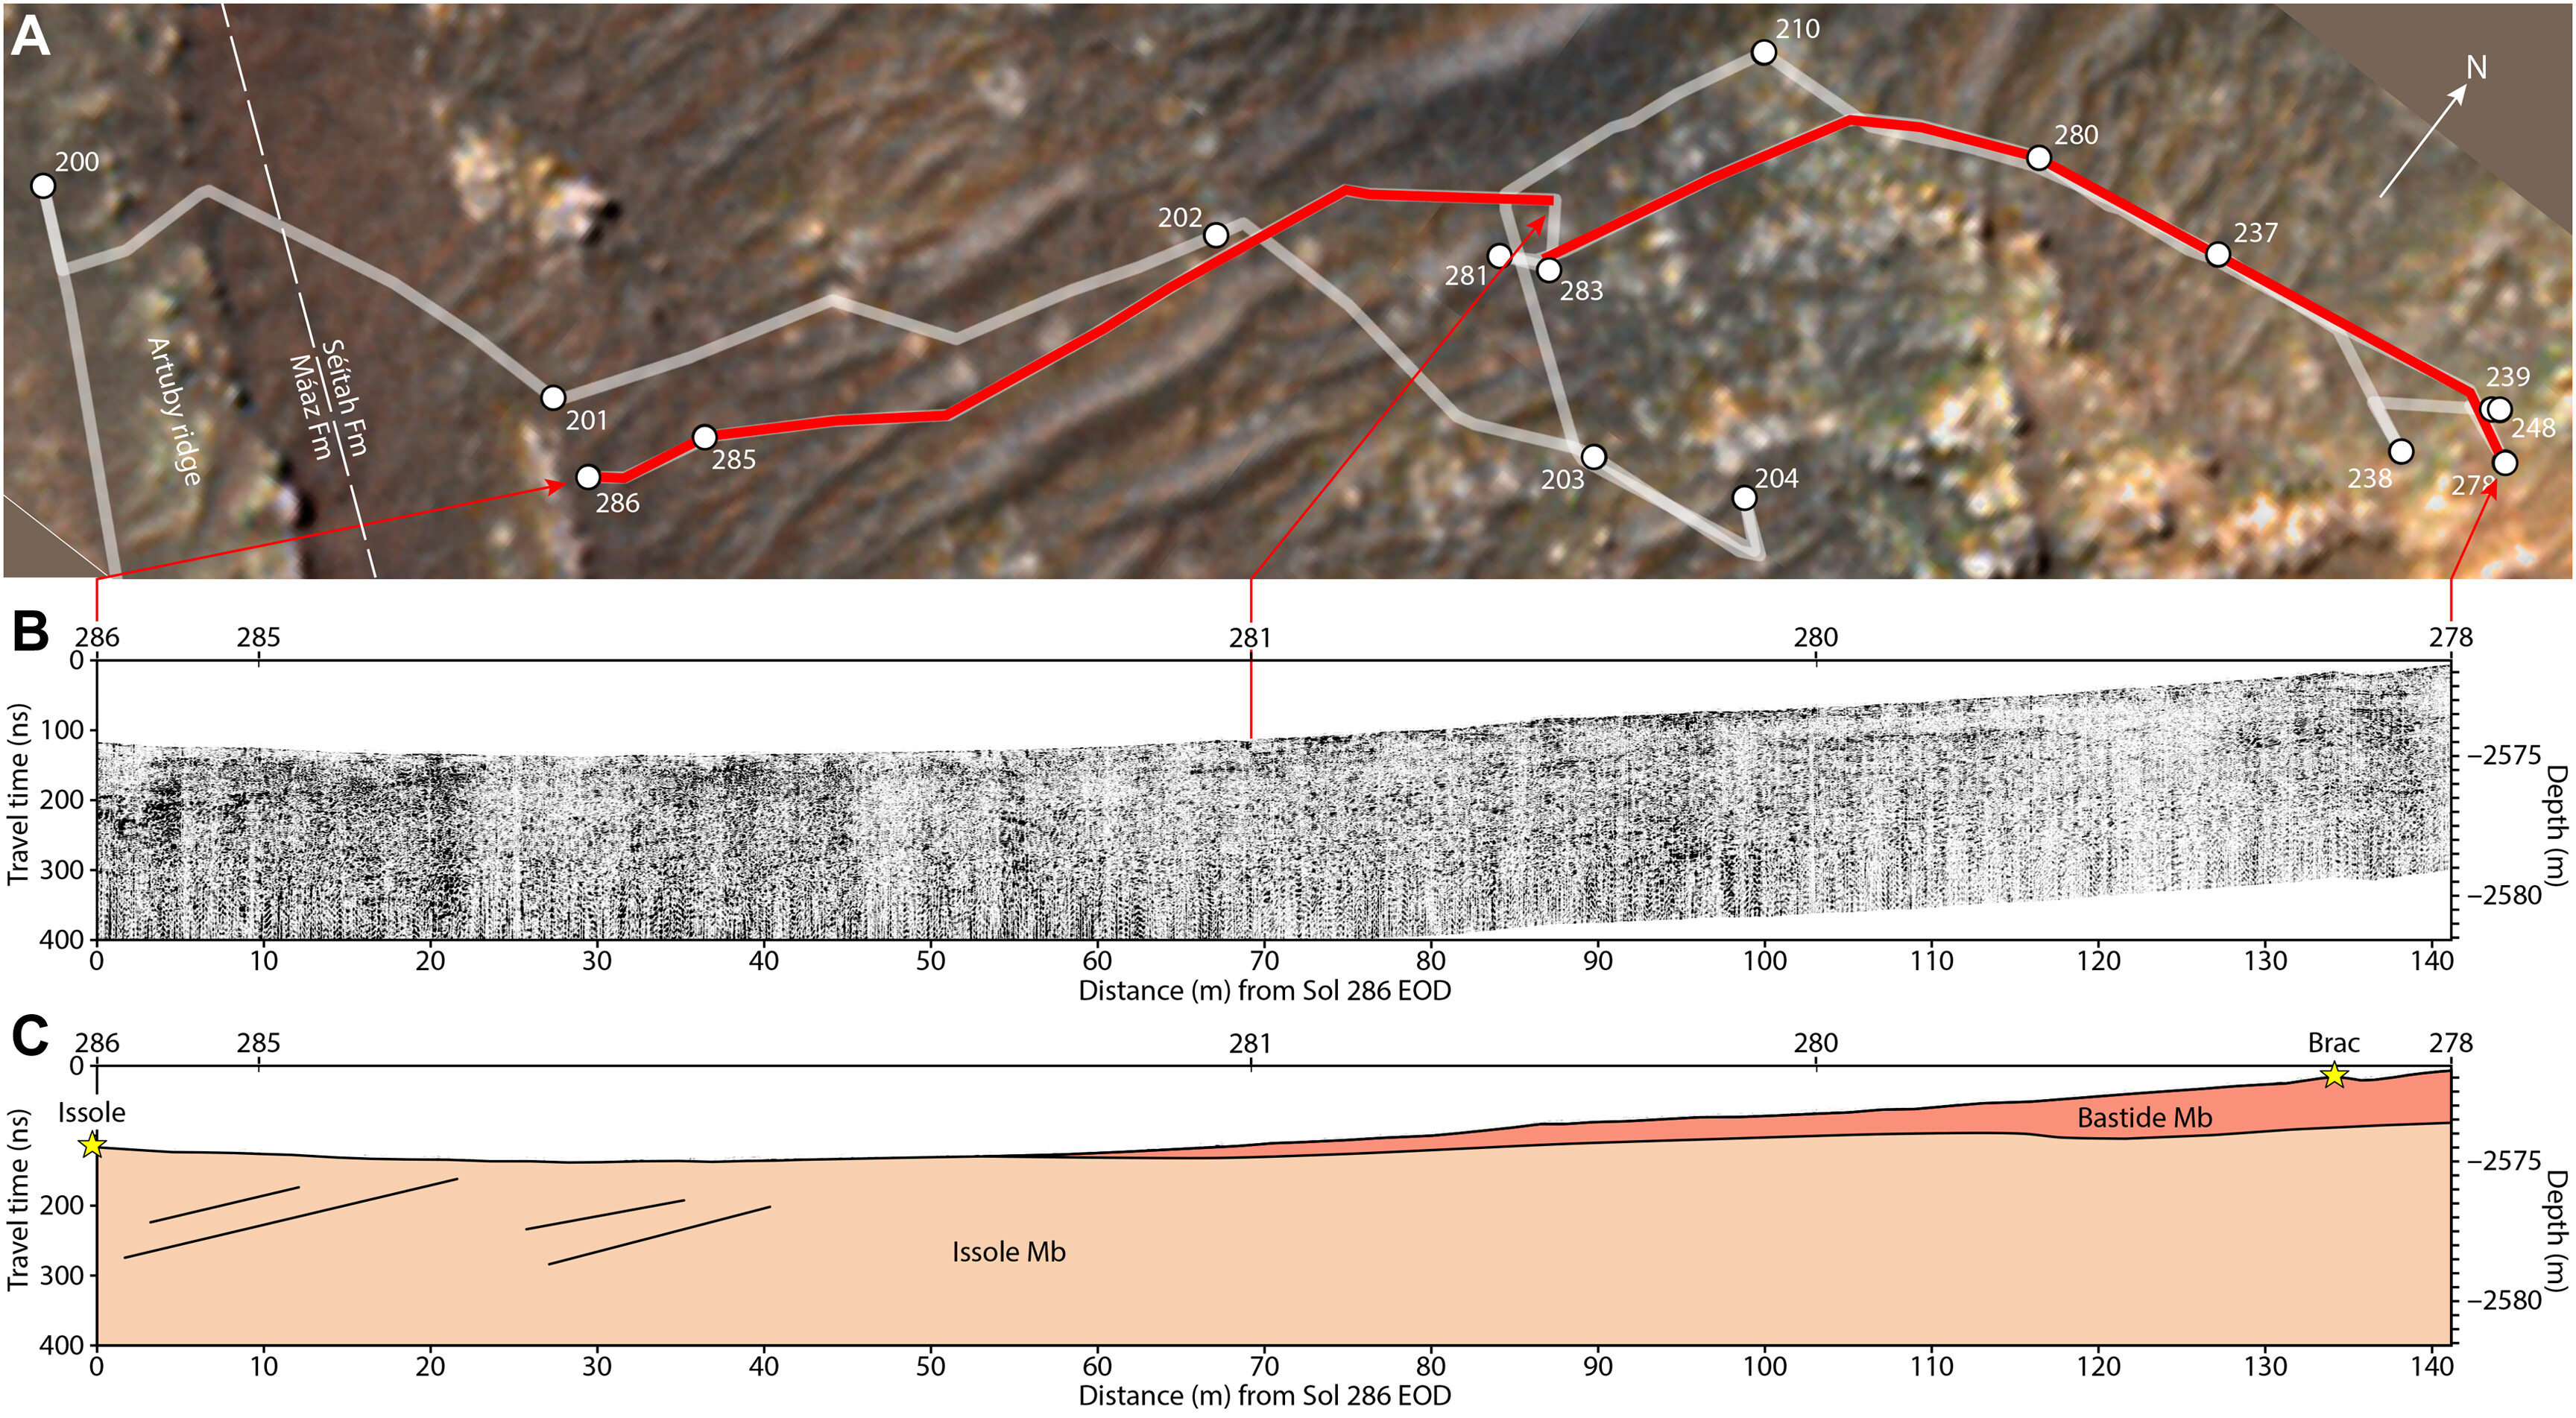
\includegraphics[width=0.9\linewidth]{Figures/0.5RIMFAX/Hamran_2022-f3.jpg}
    \caption[RIMFAX transition between two packages from sol 278 to 286]{RIMFAX transition between two packages from sol 278 to 286 \citep{Hamran2022}. \textbf{Keywords:} Strongly dipping reflectors, truncating reflections, clinoform structures, continuous to discontinuous, high to low reflectivity.}
    \label{fig:Hamran22-3}
\end{figure}

\begin{figure}[h!]
    \centering
    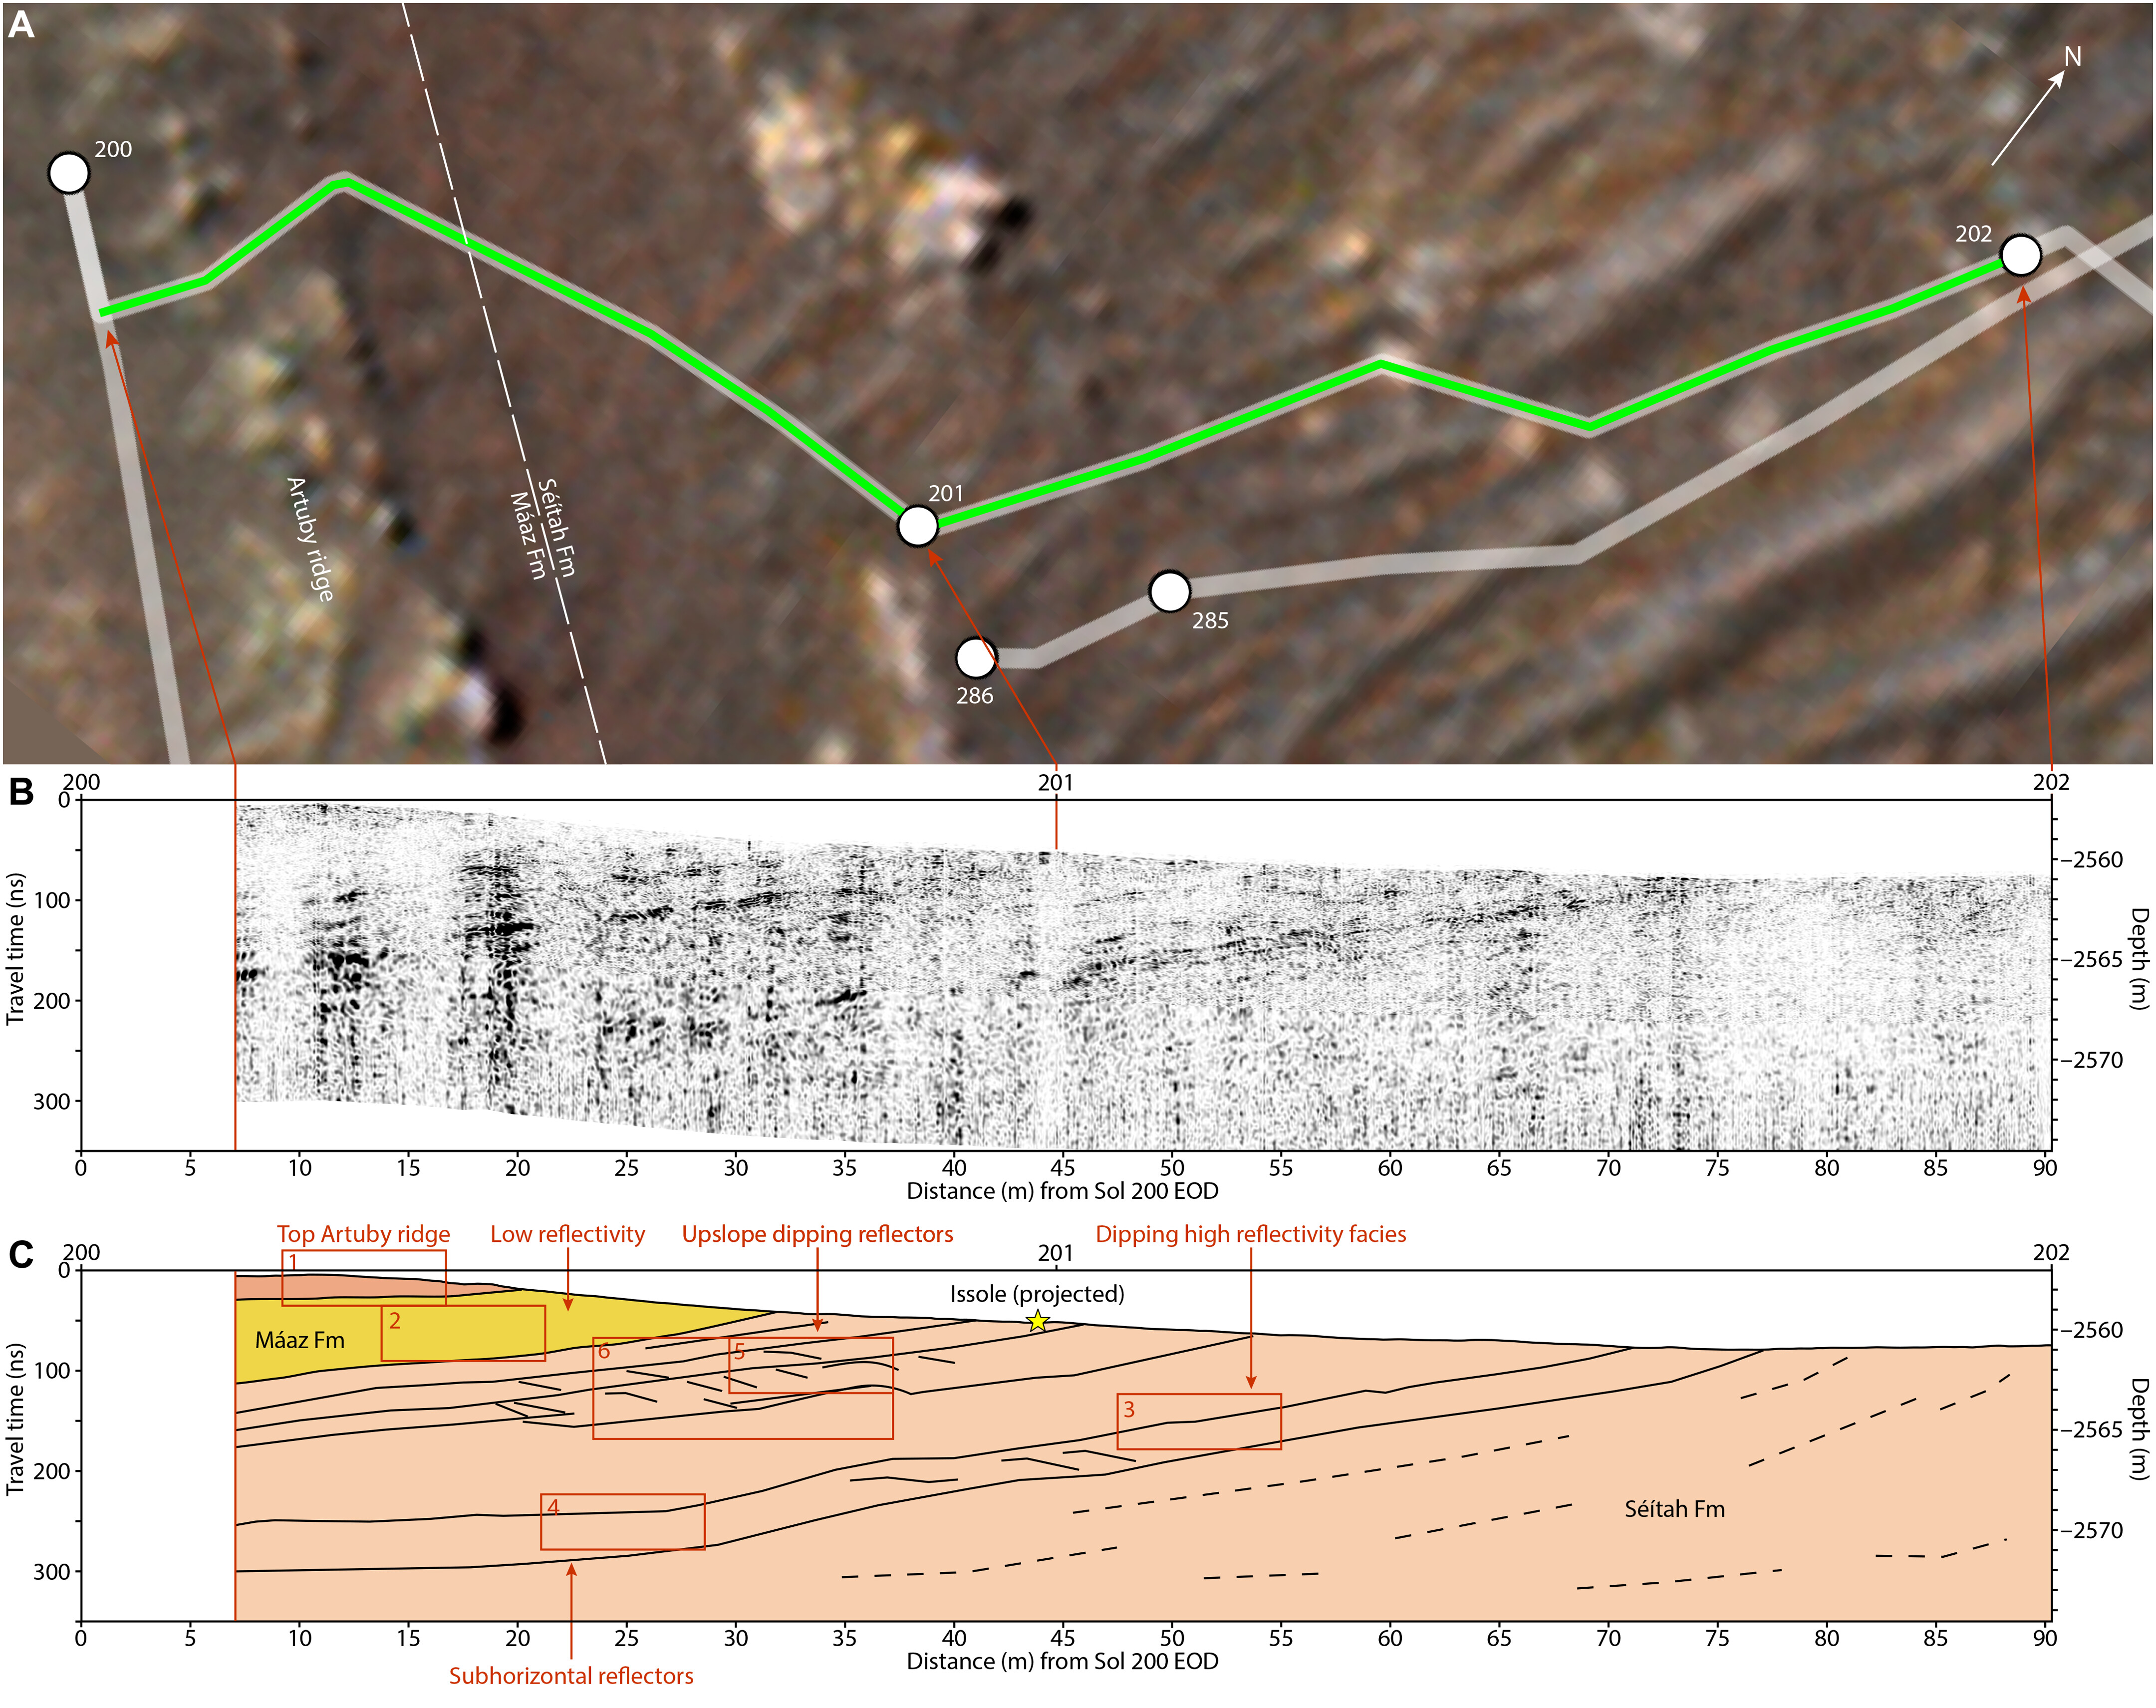
\includegraphics[width=0.9\linewidth]{Figures/0.5RIMFAX/Hamran_2022-f4.jpg}
    \caption[RIMFAX radargram acquired from Sol 201 and Sol 202.]{RIMFAX radargram acquired from Sol 201 and Sol 202 \citep{Hamran2022}. \textbf{Keywords:} Attenuated signal, radar-transparent zones, sparse internal reflections, dipping layers, semi-layered, multidirectional dipping, discontinuous layers, semi-continuous layers.}
    \label{fig:Hamran22-4}
\end{figure}

\begin{figure}
    \centering
    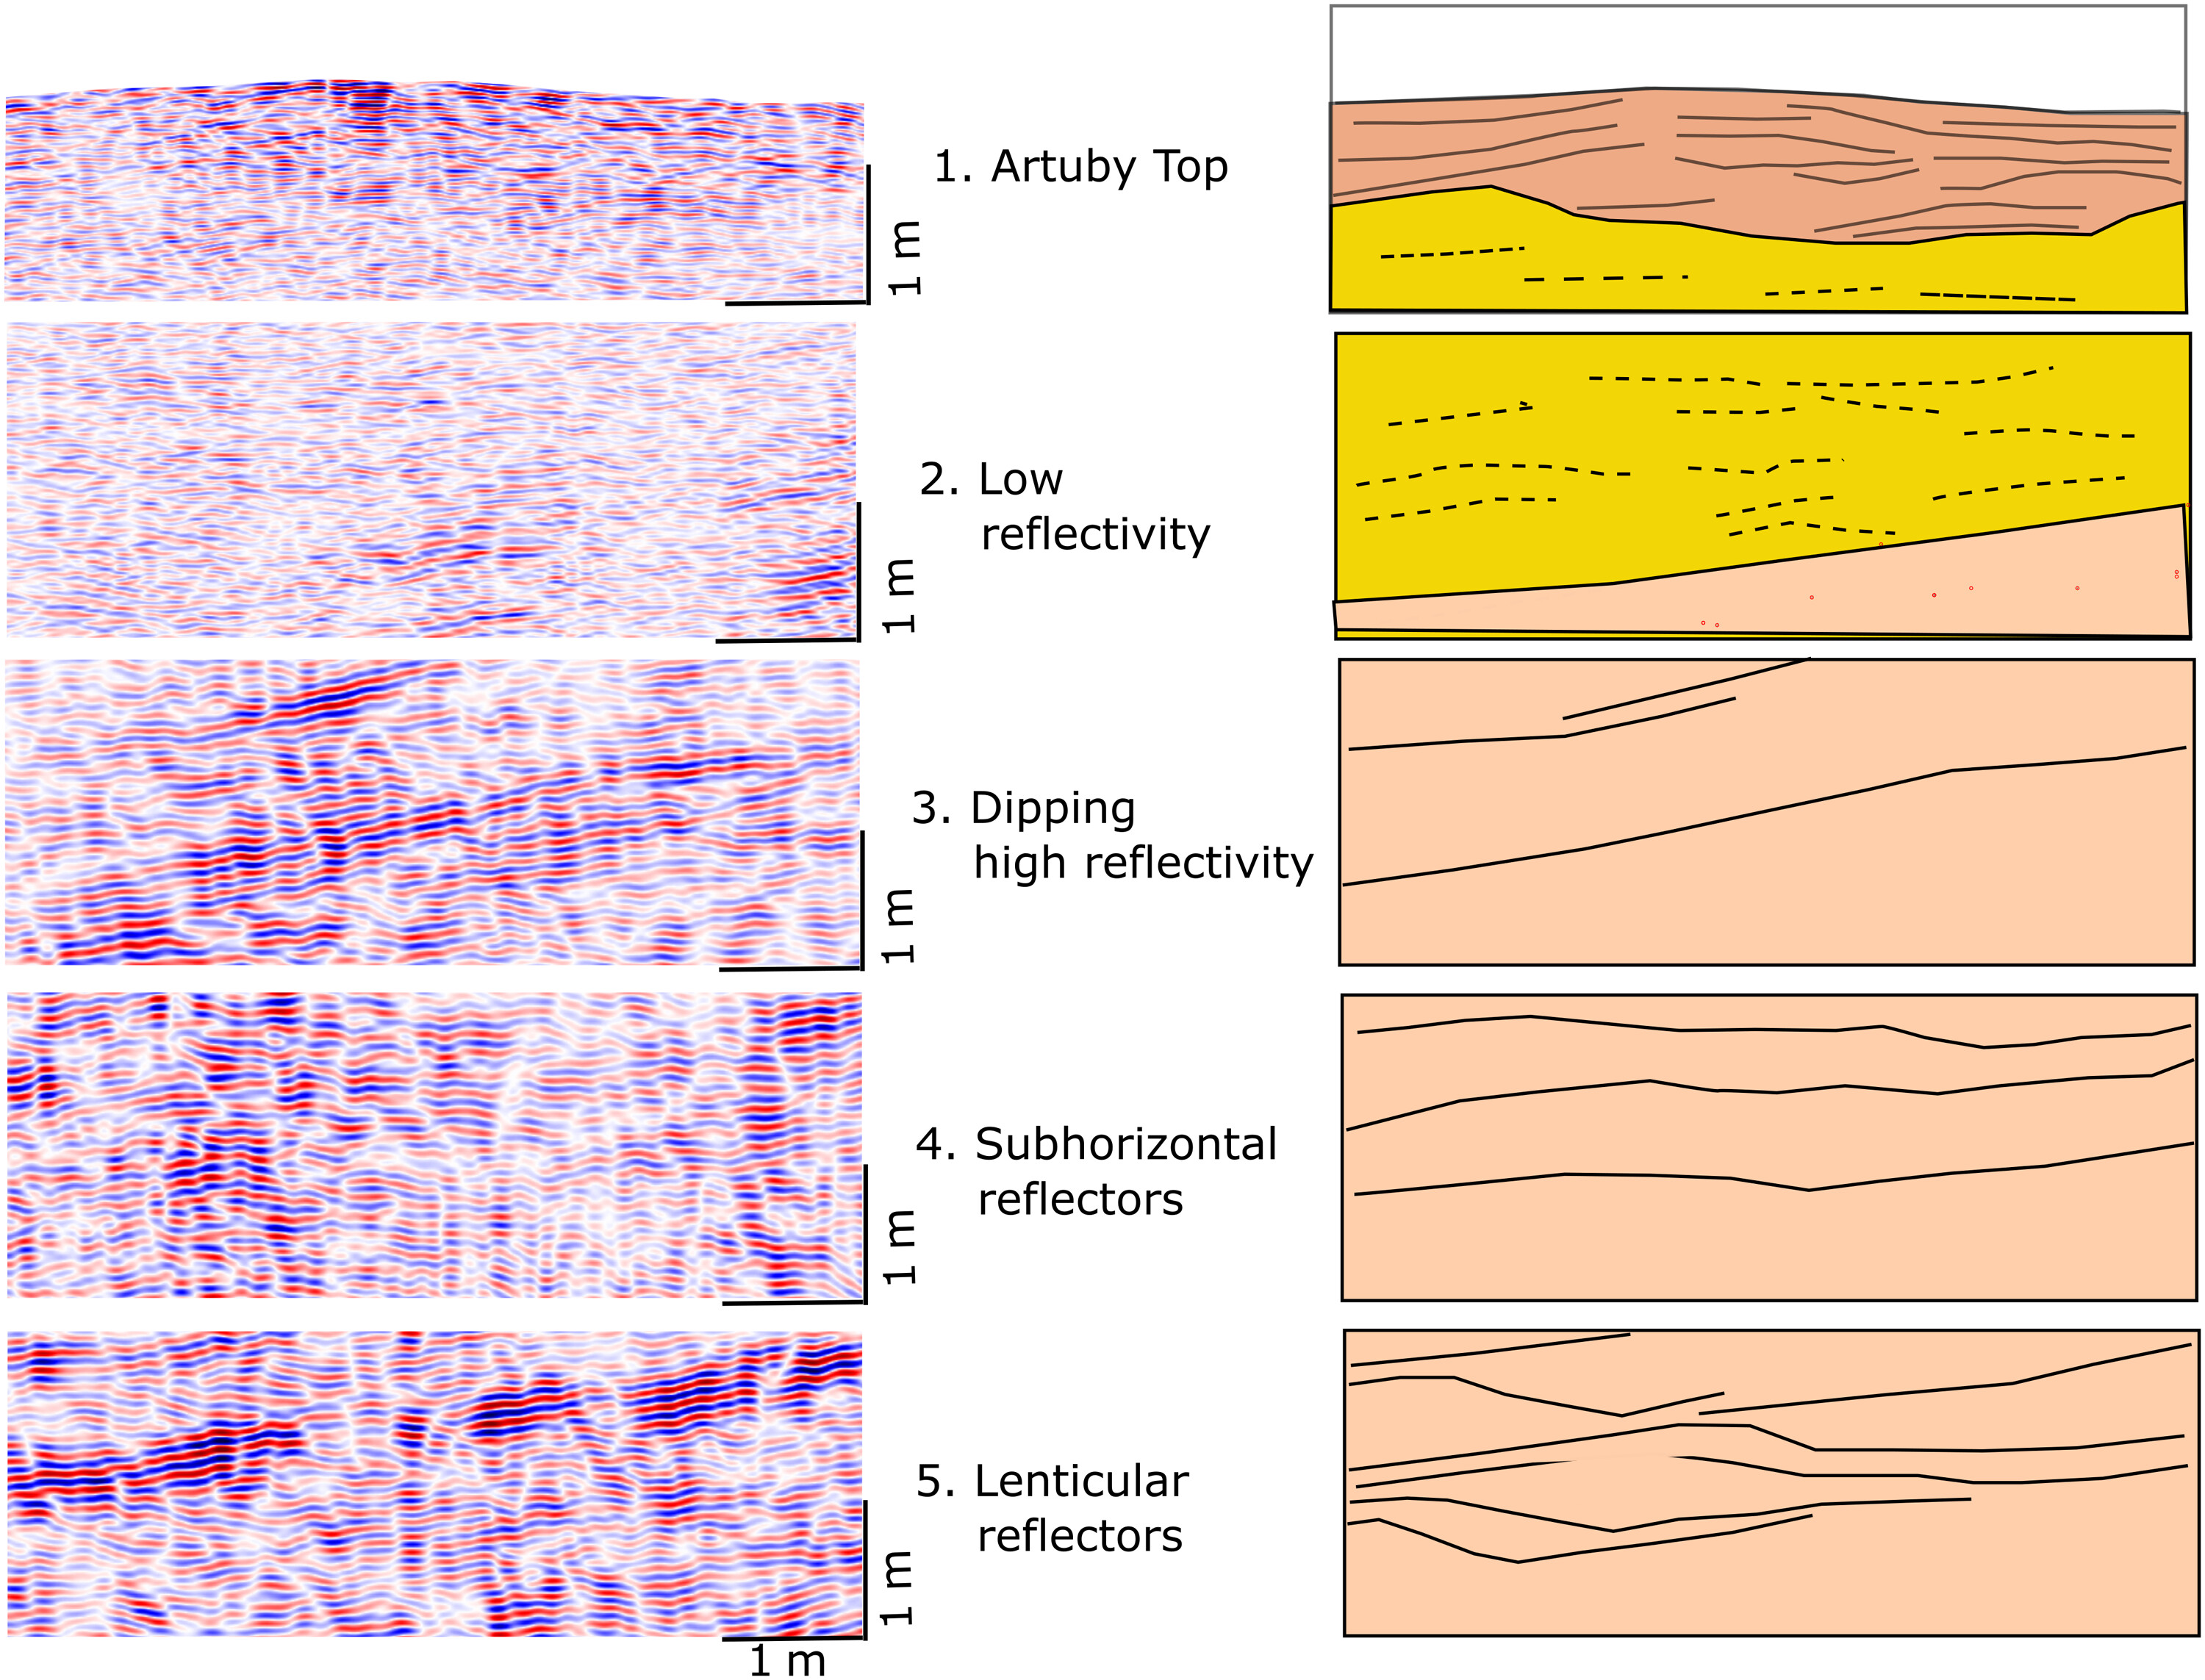
\includegraphics[width=0.9\linewidth]{Figures/0.5RIMFAX/Hamran_2022-f5.jpg}
    \caption[RIMFAX radar facies observed during Sol 201 and Sol 202.]{RIMFAX radar facies observed during Sol 201 and Sol 202 \citep{Hamran2022}. \textbf{Keywords:} Coherent near-surface layering, subparallel, low reflectivity, high reflectivity, dipping layers, parallel, sub-horizontal, lenticular reflectors, sigmoidal profiles.}
    \label{fig:Hamran22-5}
\end{figure}

\clearpage

\begin{figure}[h!]
    \centering
    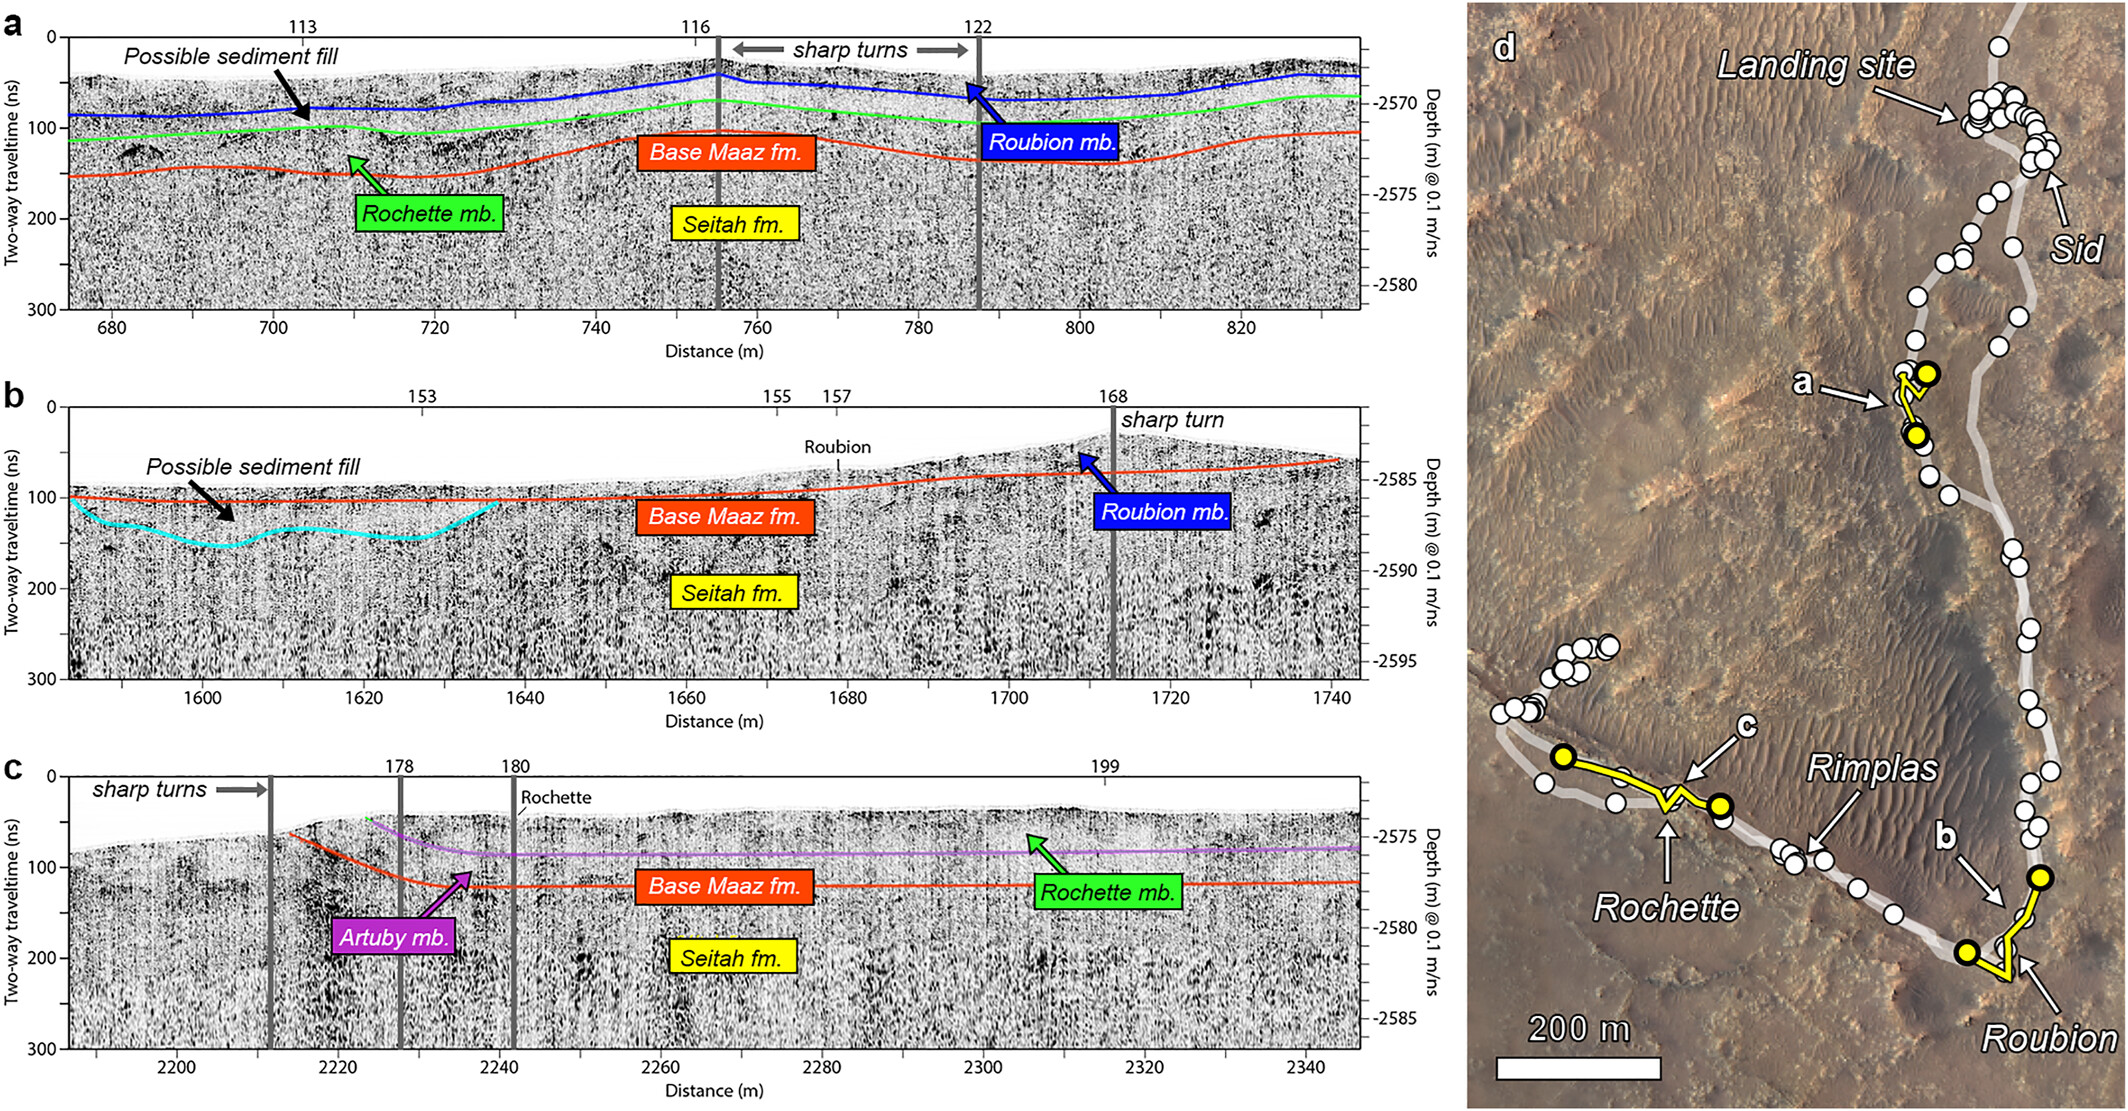
\includegraphics[width=0.9\linewidth]{Figures/0.5RIMFAX/Horgan_2023-fig1.jpg}
    \caption[RIMFAX traverse from sol 112–123.]{RIMFAX traverse from sol 112–123 \citep{Horgan2023}. \textbf{Keywords:} Strong surface reflections, transparent unit, low-density fill, low reflectivity, chaotic.}
    \label{fig:Horgan23-1}
\end{figure}

\begin{figure}[h!]
    \centering
    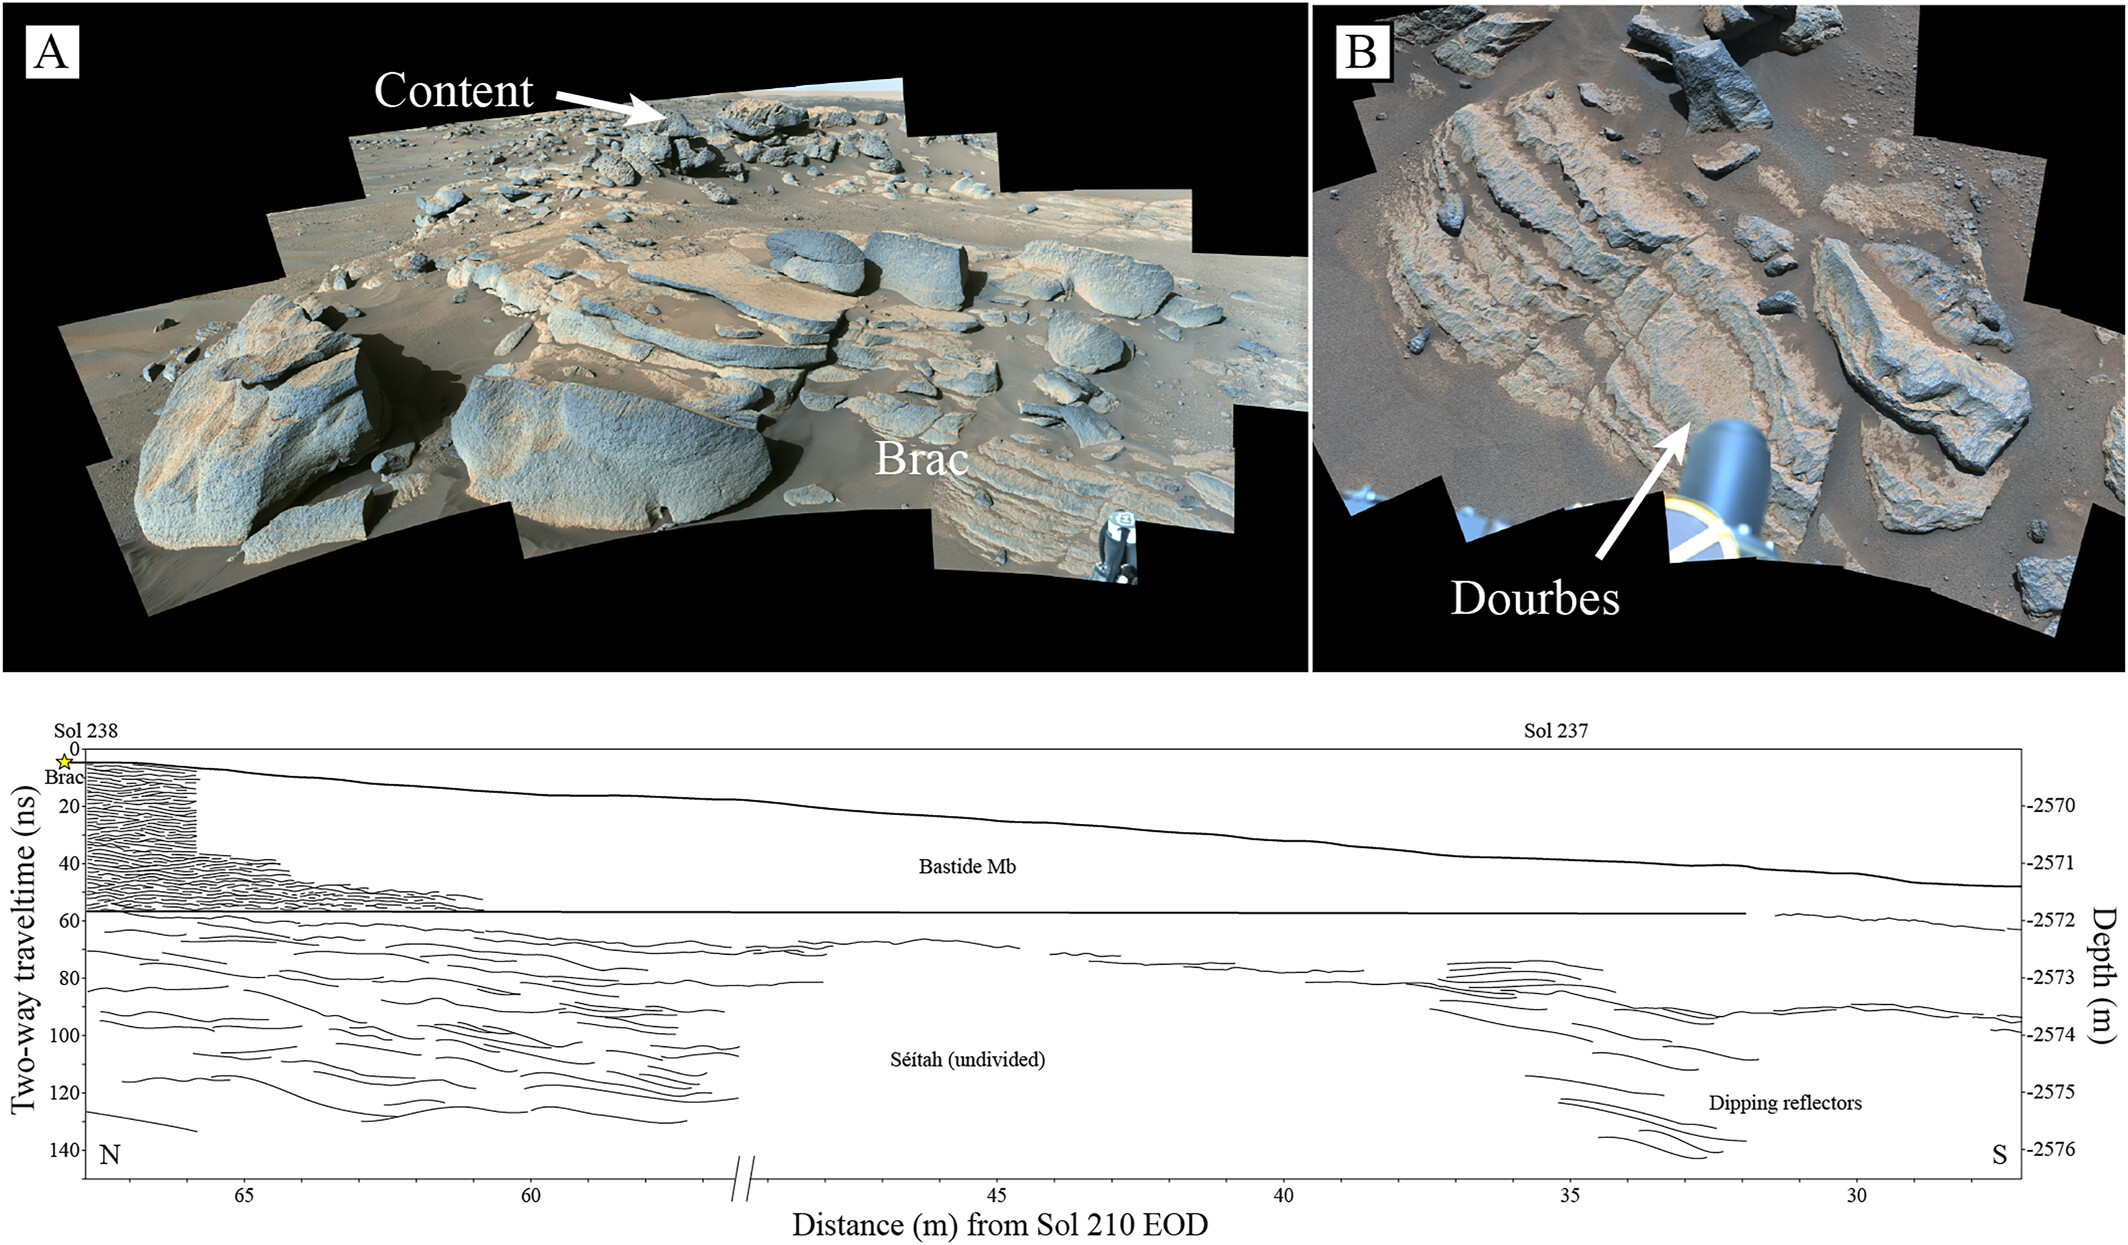
\includegraphics[width=0.9\linewidth]{Figures/0.5RIMFAX/Simon_2023-fig-03.jpg}
    \caption[RIMFAX traverse from sol 210]{RIMFAX traverse from sol 210 \citep{Simon2023}. \textbf{Keywords: } Sloped-surface, discontinuous, dipping, lenticulars.}
    \label{fig:Simon23-3}
\end{figure}
 
\begin{figure}[h!]
    \centering
    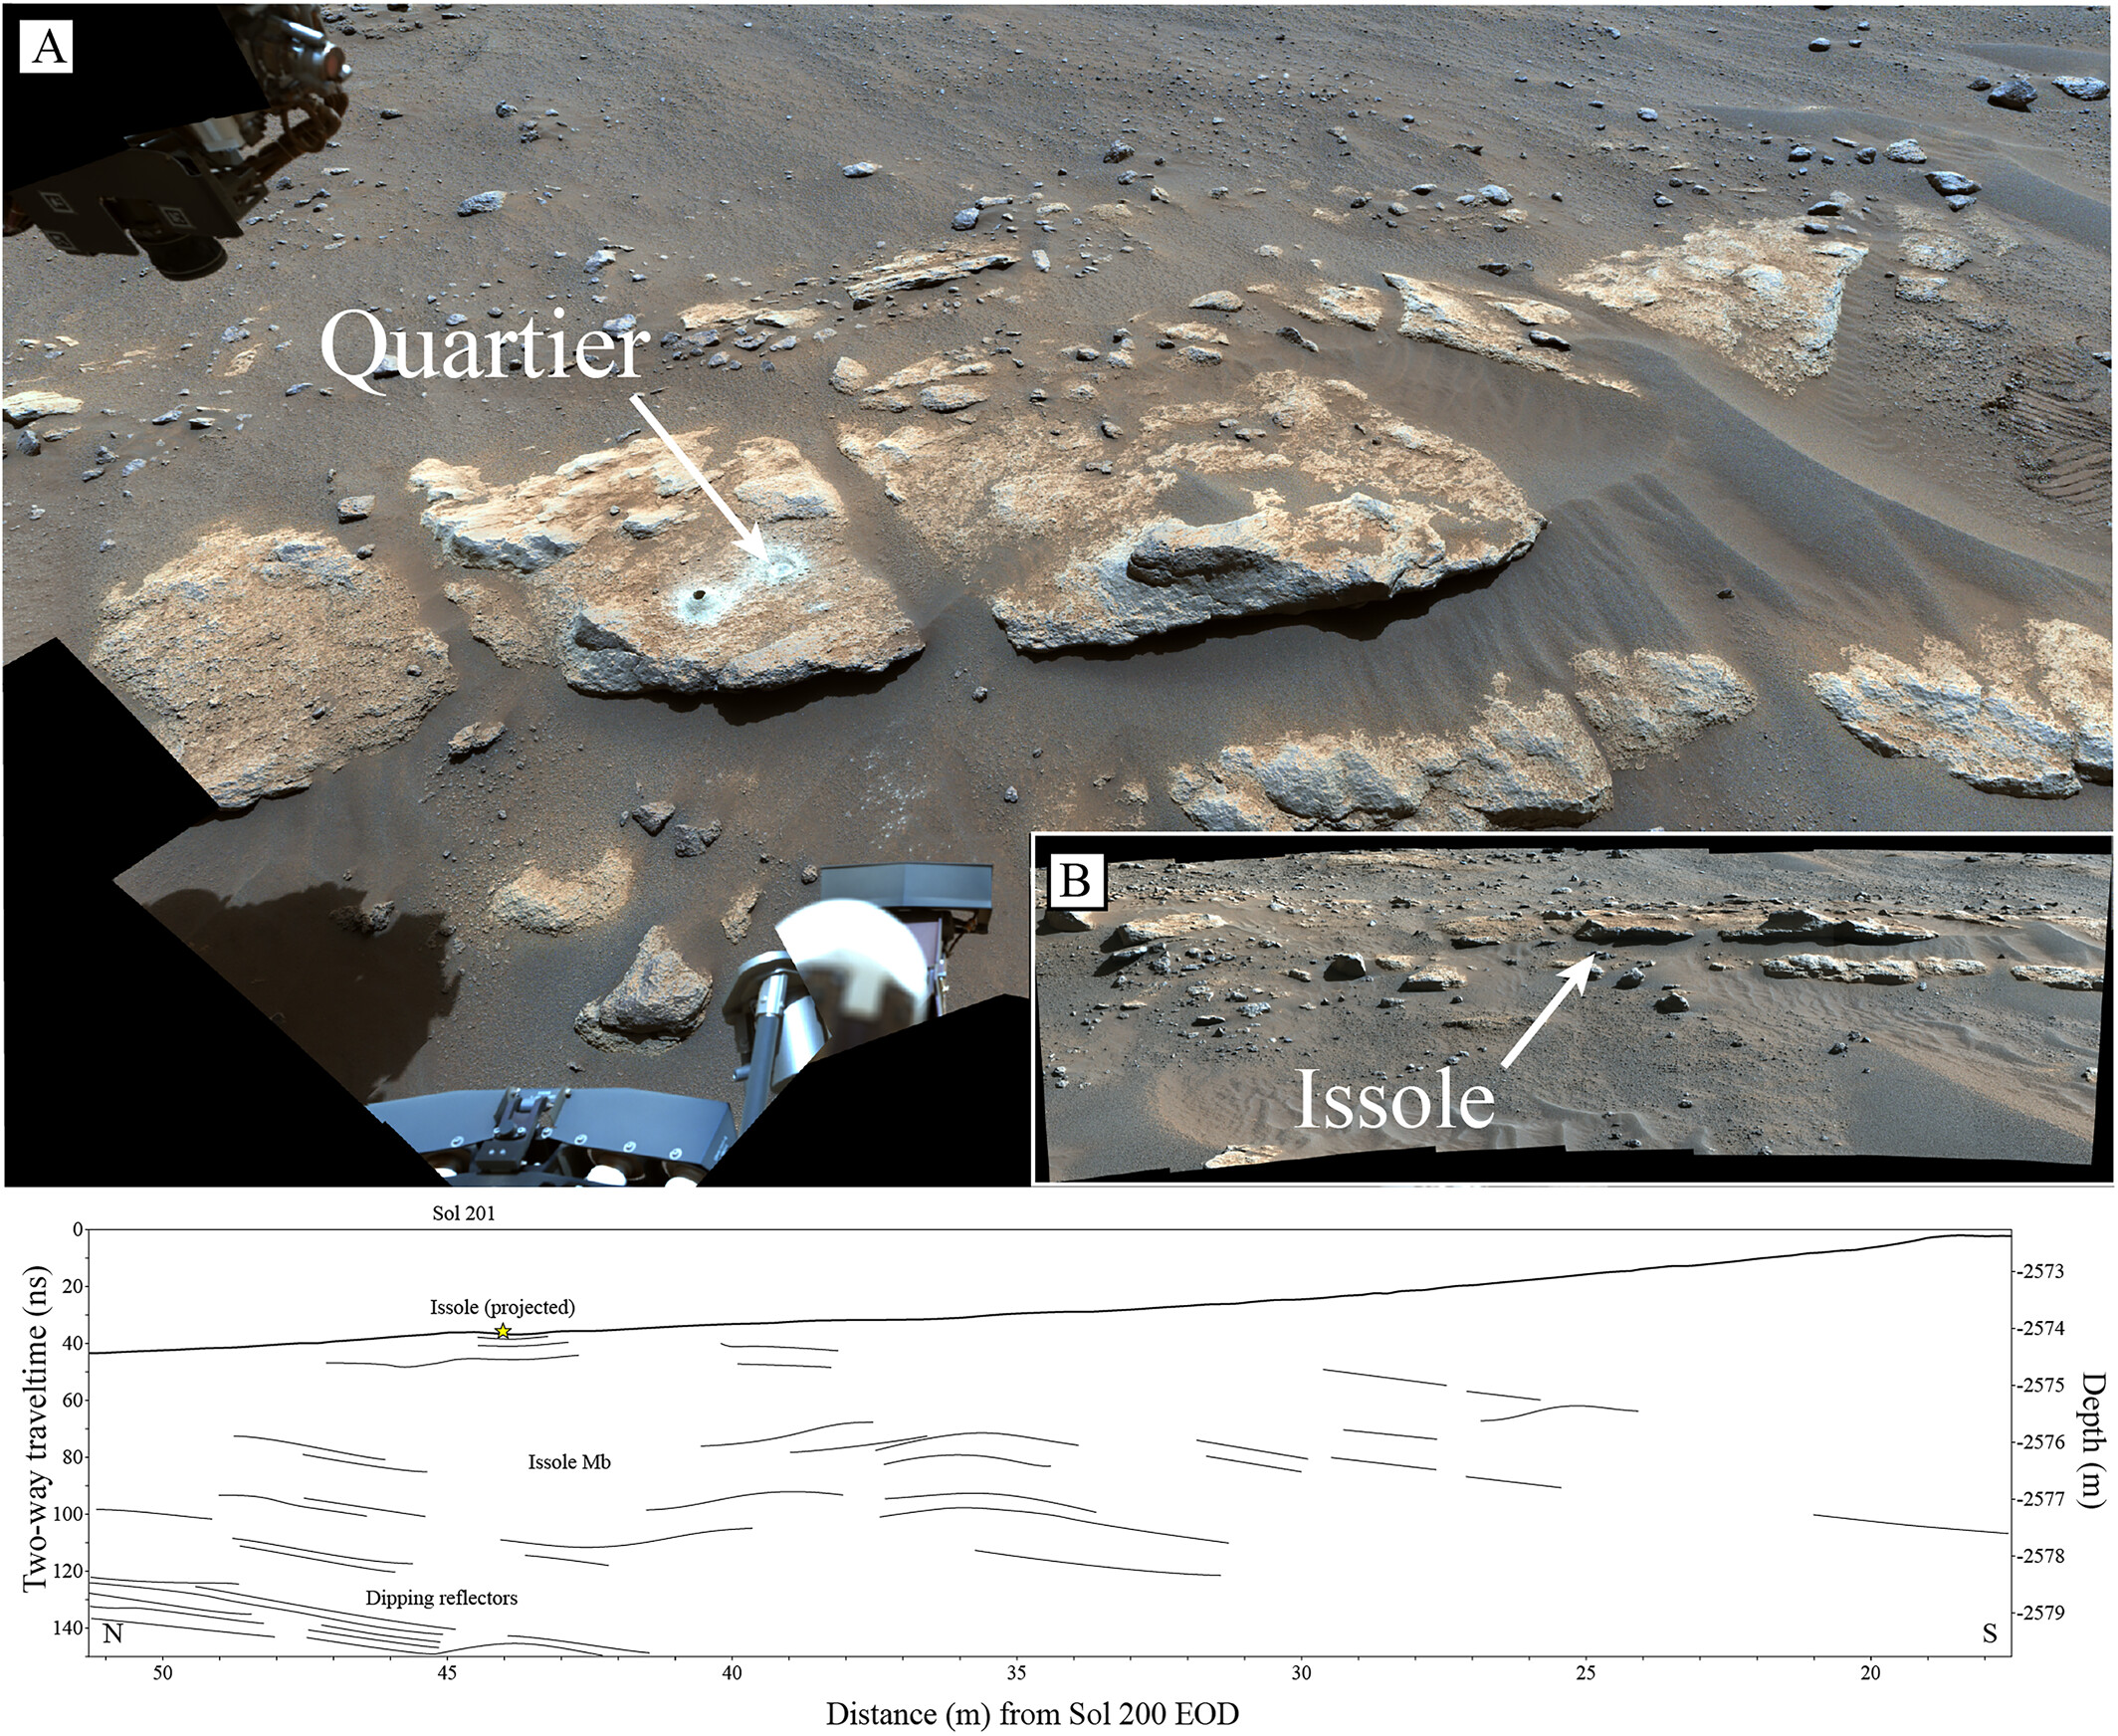
\includegraphics[width=0.9\linewidth]{Figures/0.5RIMFAX/Simon_2023-fig-04.jpg}
    \caption[RIMFAX Sol 200.]{RIMFAX Sol 200 \citep{Simon2023}. \textbf{Keywords:} Multi-directional dipping, semi-continuous, low continuity, ridge.}
    \label{fig:Simon23-4}
\end{figure}

\begin{figure}[h!]
    \centering
    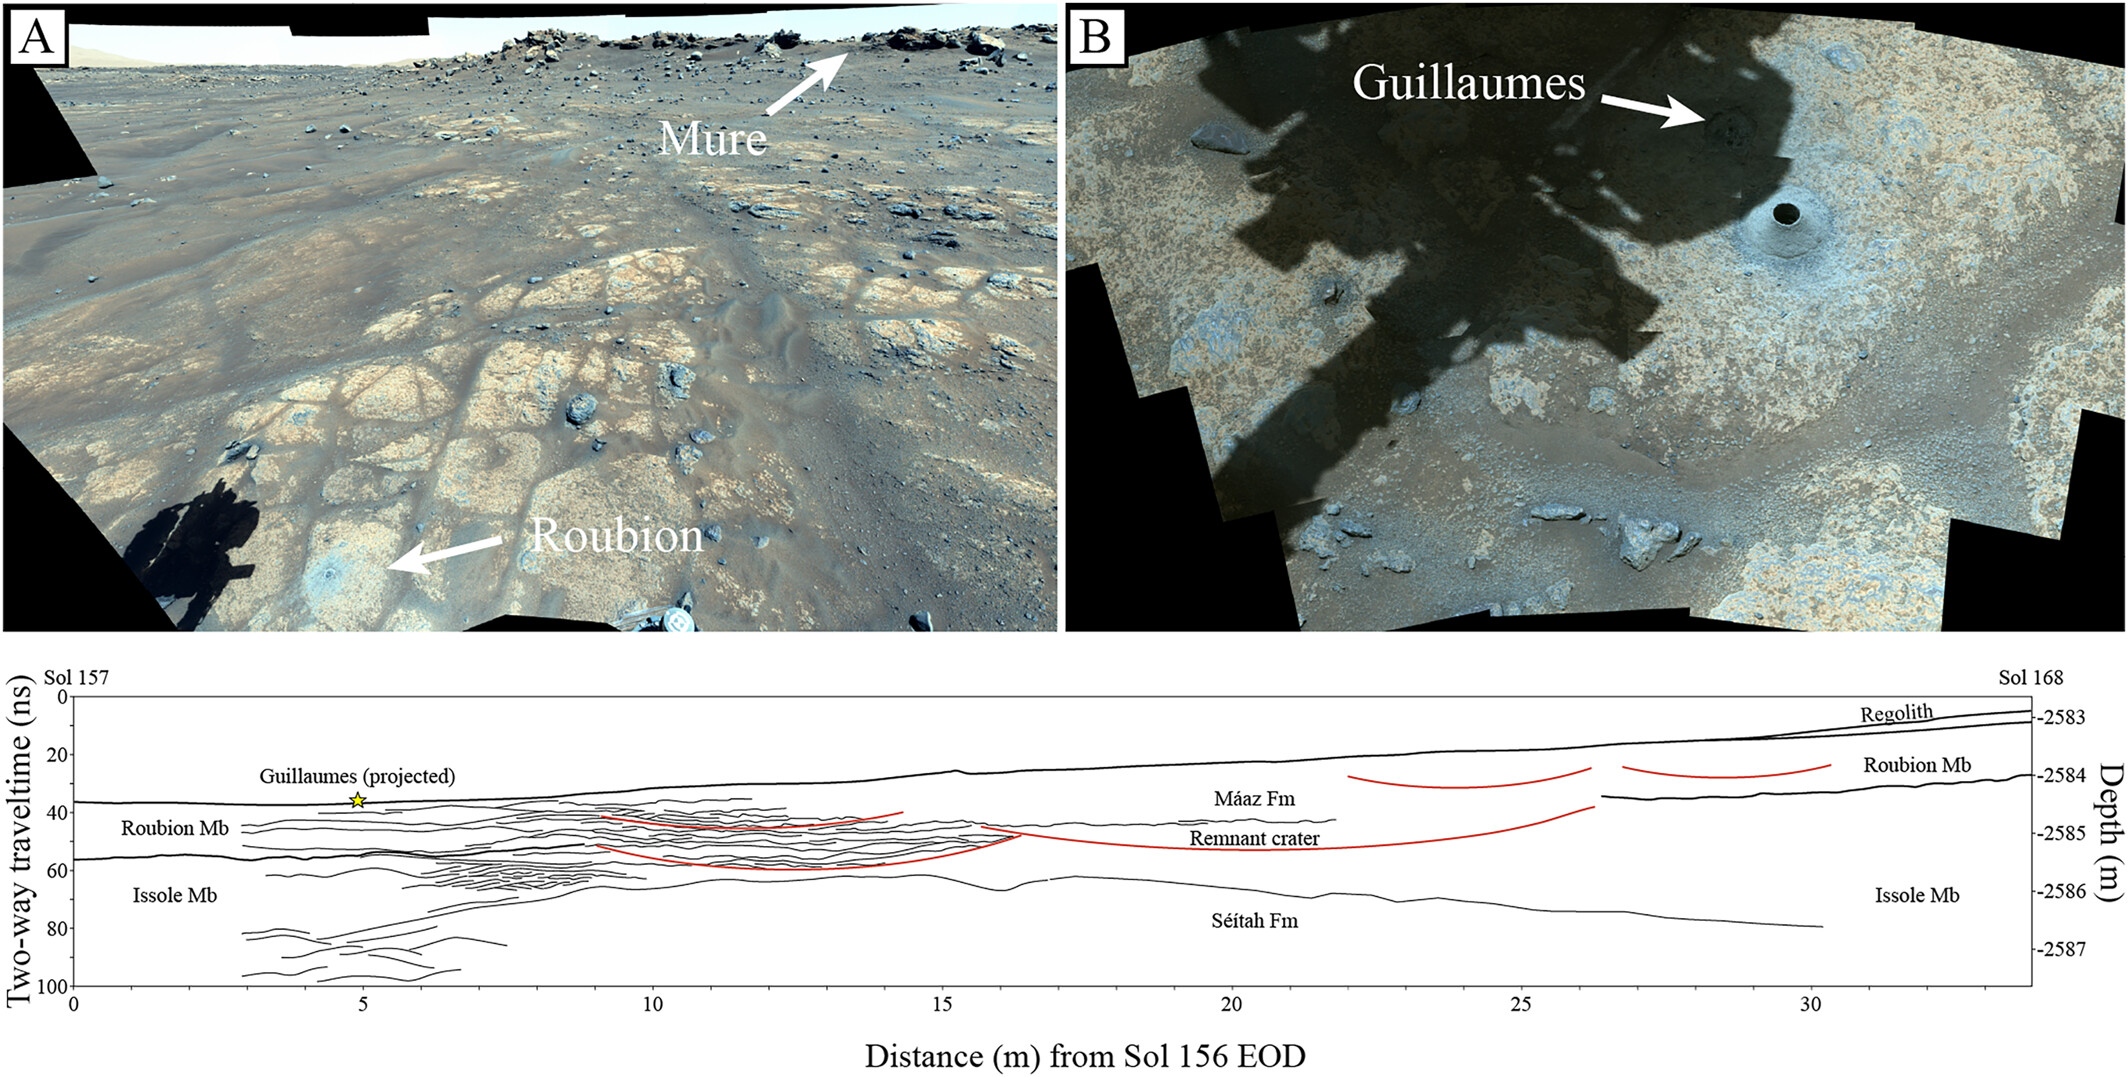
\includegraphics[width=0.9\linewidth]{Figures/0.5RIMFAX/Simon_2023-fig-05.jpg}
    \caption[RIMFAX traverse from sol 156]{RIMFAX traverse from sol 156 \citep{Simon2023}. \textbf{Keywords:}Semi-horizontal, hummocky, lenticulars, crossing reflectors, semi-continuous, low reflectivity, high reflectivity, multi-directional dipping. }
    \label{fig:Simon23-5}
\end{figure}

\begin{figure}[h!]
    \centering
    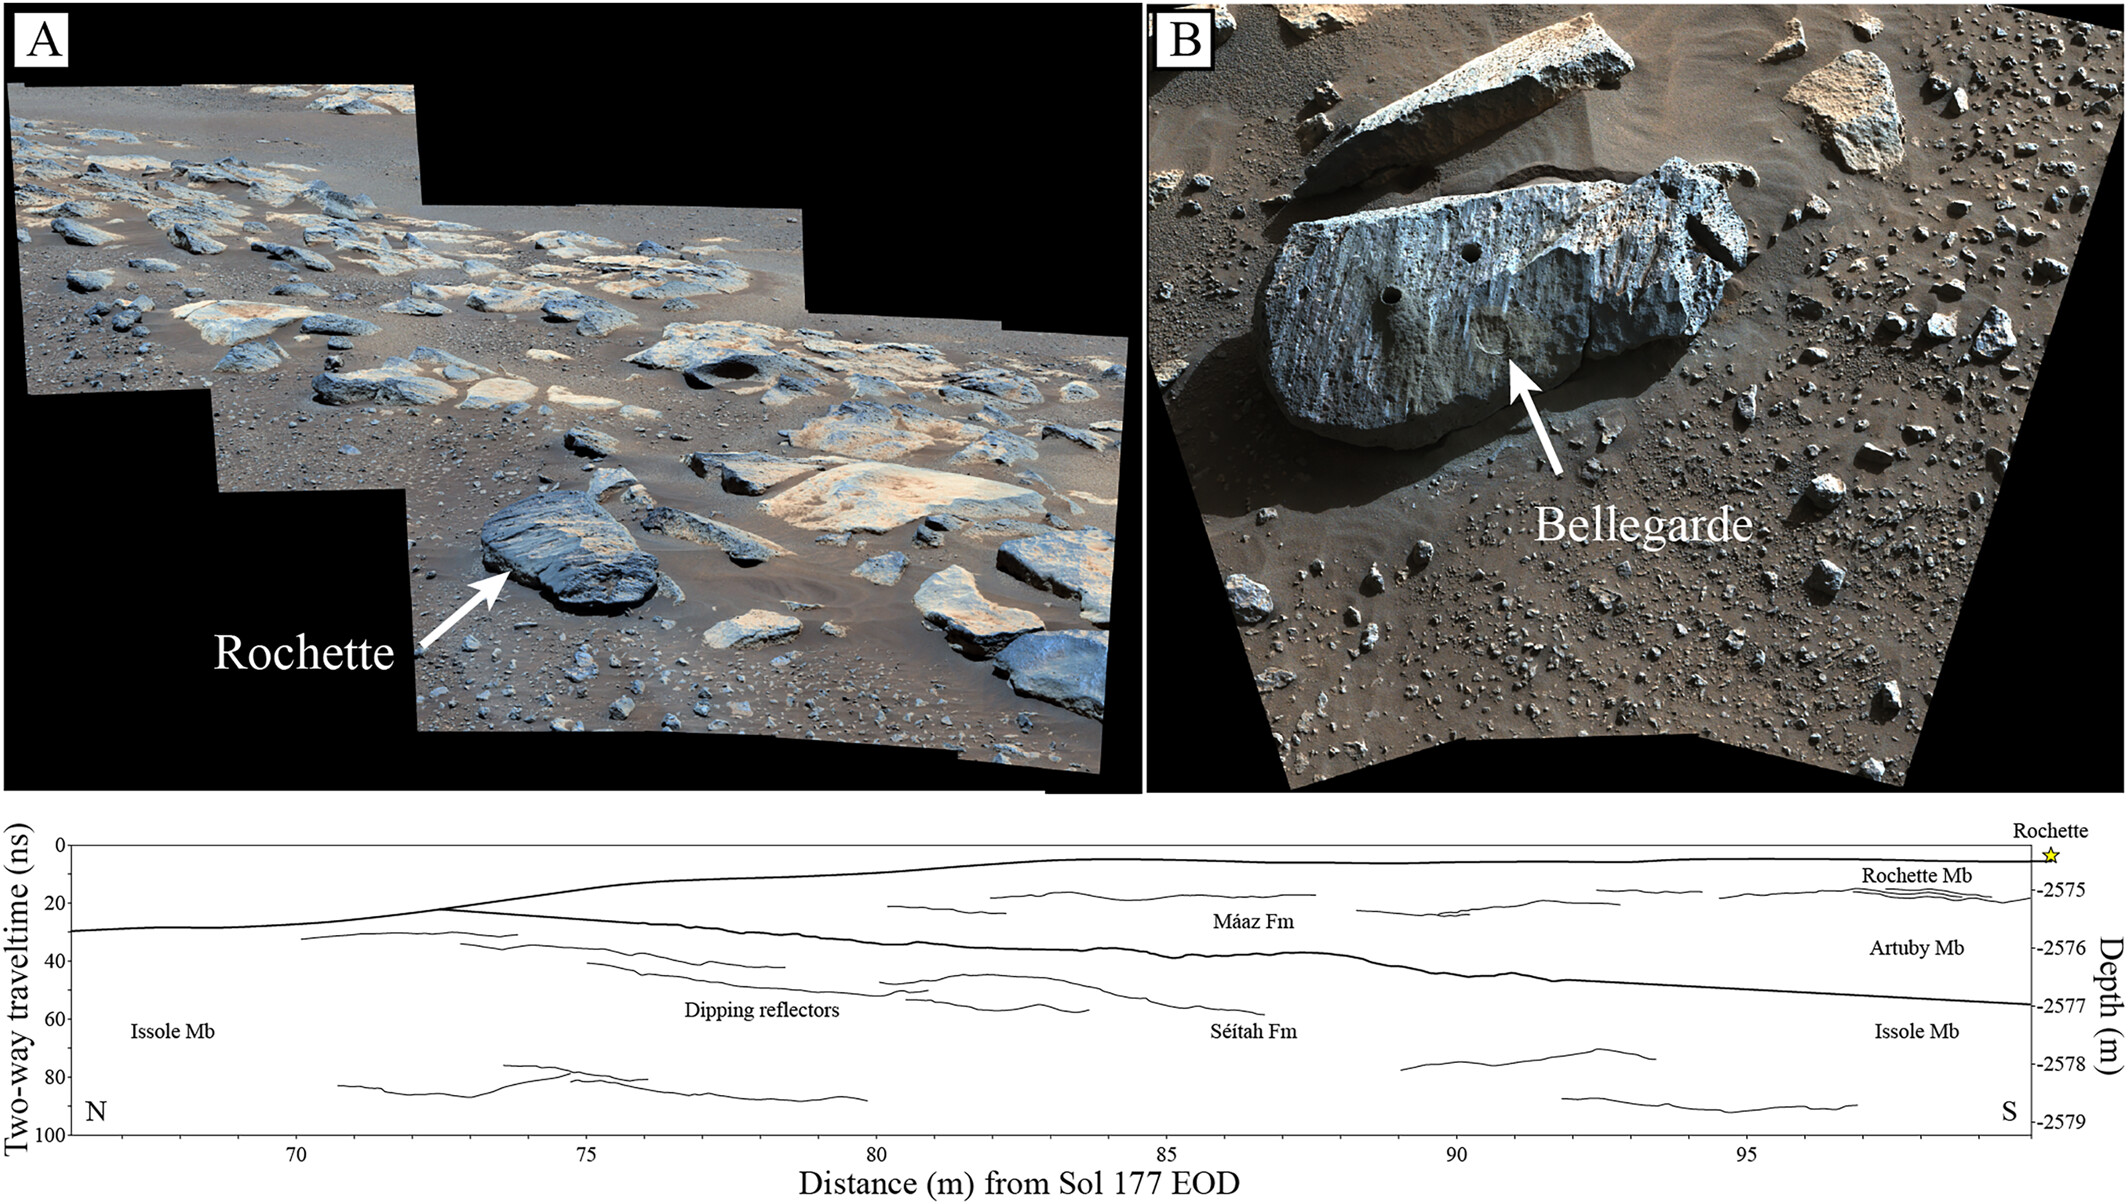
\includegraphics[width=0.9\linewidth]{Figures/0.5RIMFAX/Simon_2023-fig-06.jpg}
    \caption[RIMFAX traverse from sol 177.]{RIMFAX traverse from sol 177 \citep{Simon2023}. \textbf{Keywords:} Dipping reflectors, semi-continuous, multi-directional dipping, low reflectivity.}
    \label{fig:Simon23-6}
\end{figure}

\begin{figure}[h!]
    \centering
    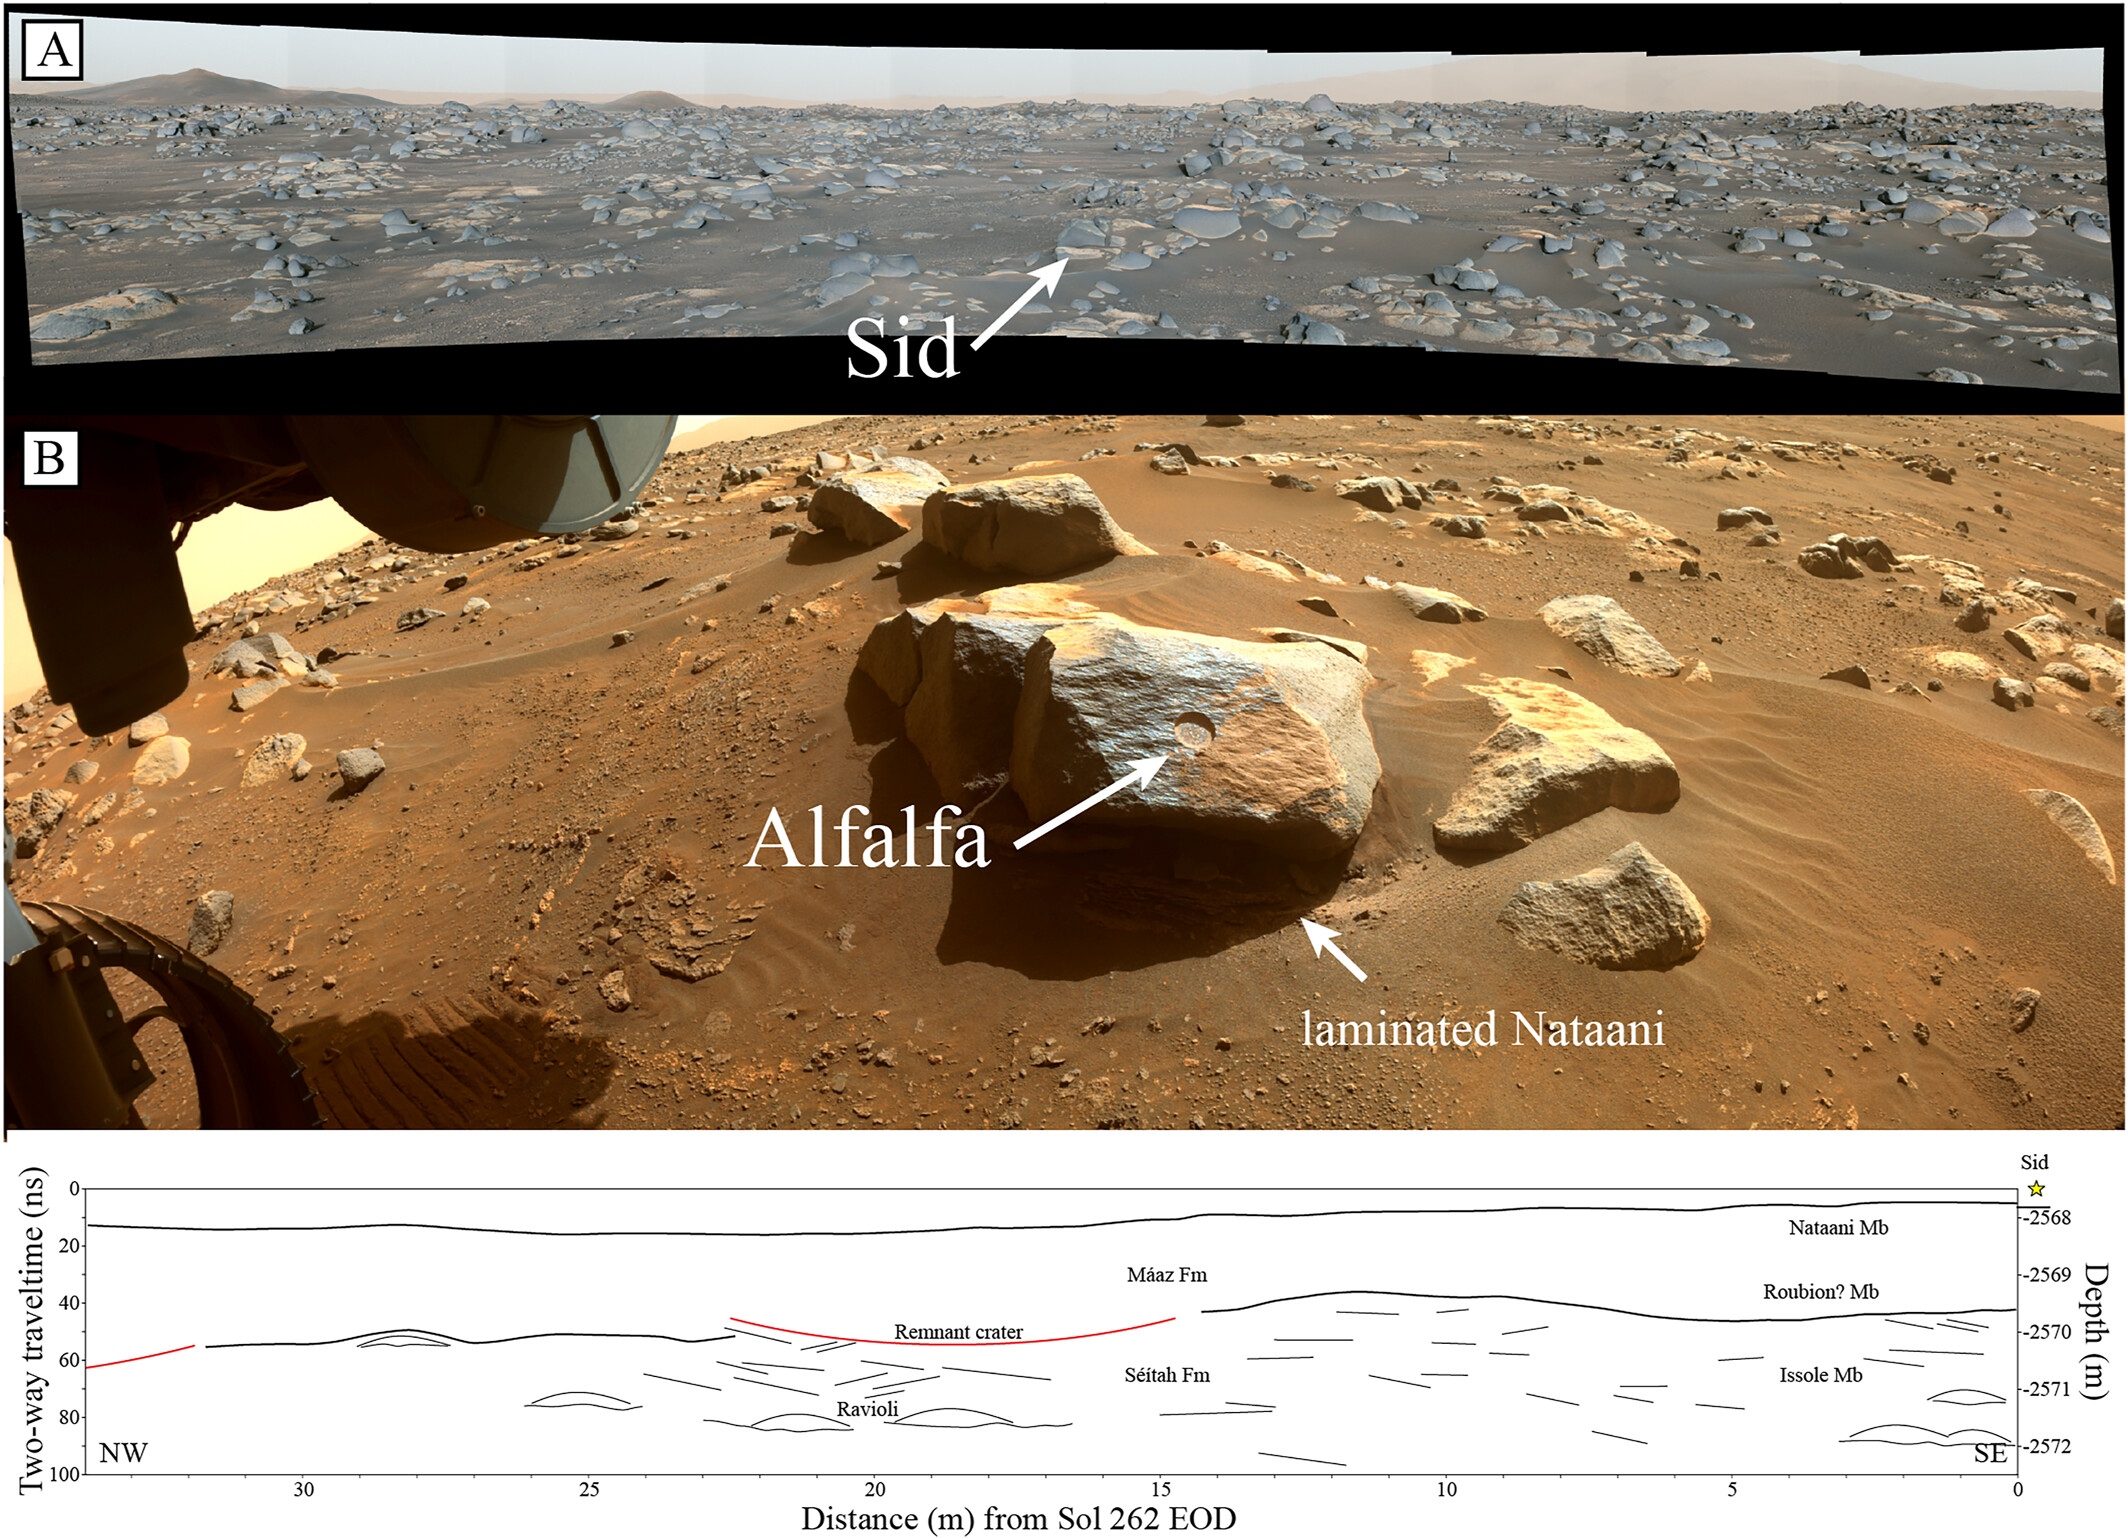
\includegraphics[width=0.9\linewidth]{Figures/0.5RIMFAX/Simon_2023-fig-07.jpg}
    \caption[RIMFAX traverse from sol 262.]{RIMFAX traverse from sol 262 \citep{Simon2023}. \textbf{Keywords:} Multi-directional dipping, low continuity, hummocky, lenticulars, horizontal layers.}
    \label{fig:Simon23-7}
\end{figure}
\clearpage
\begin{figure}[h!]
    \centering
    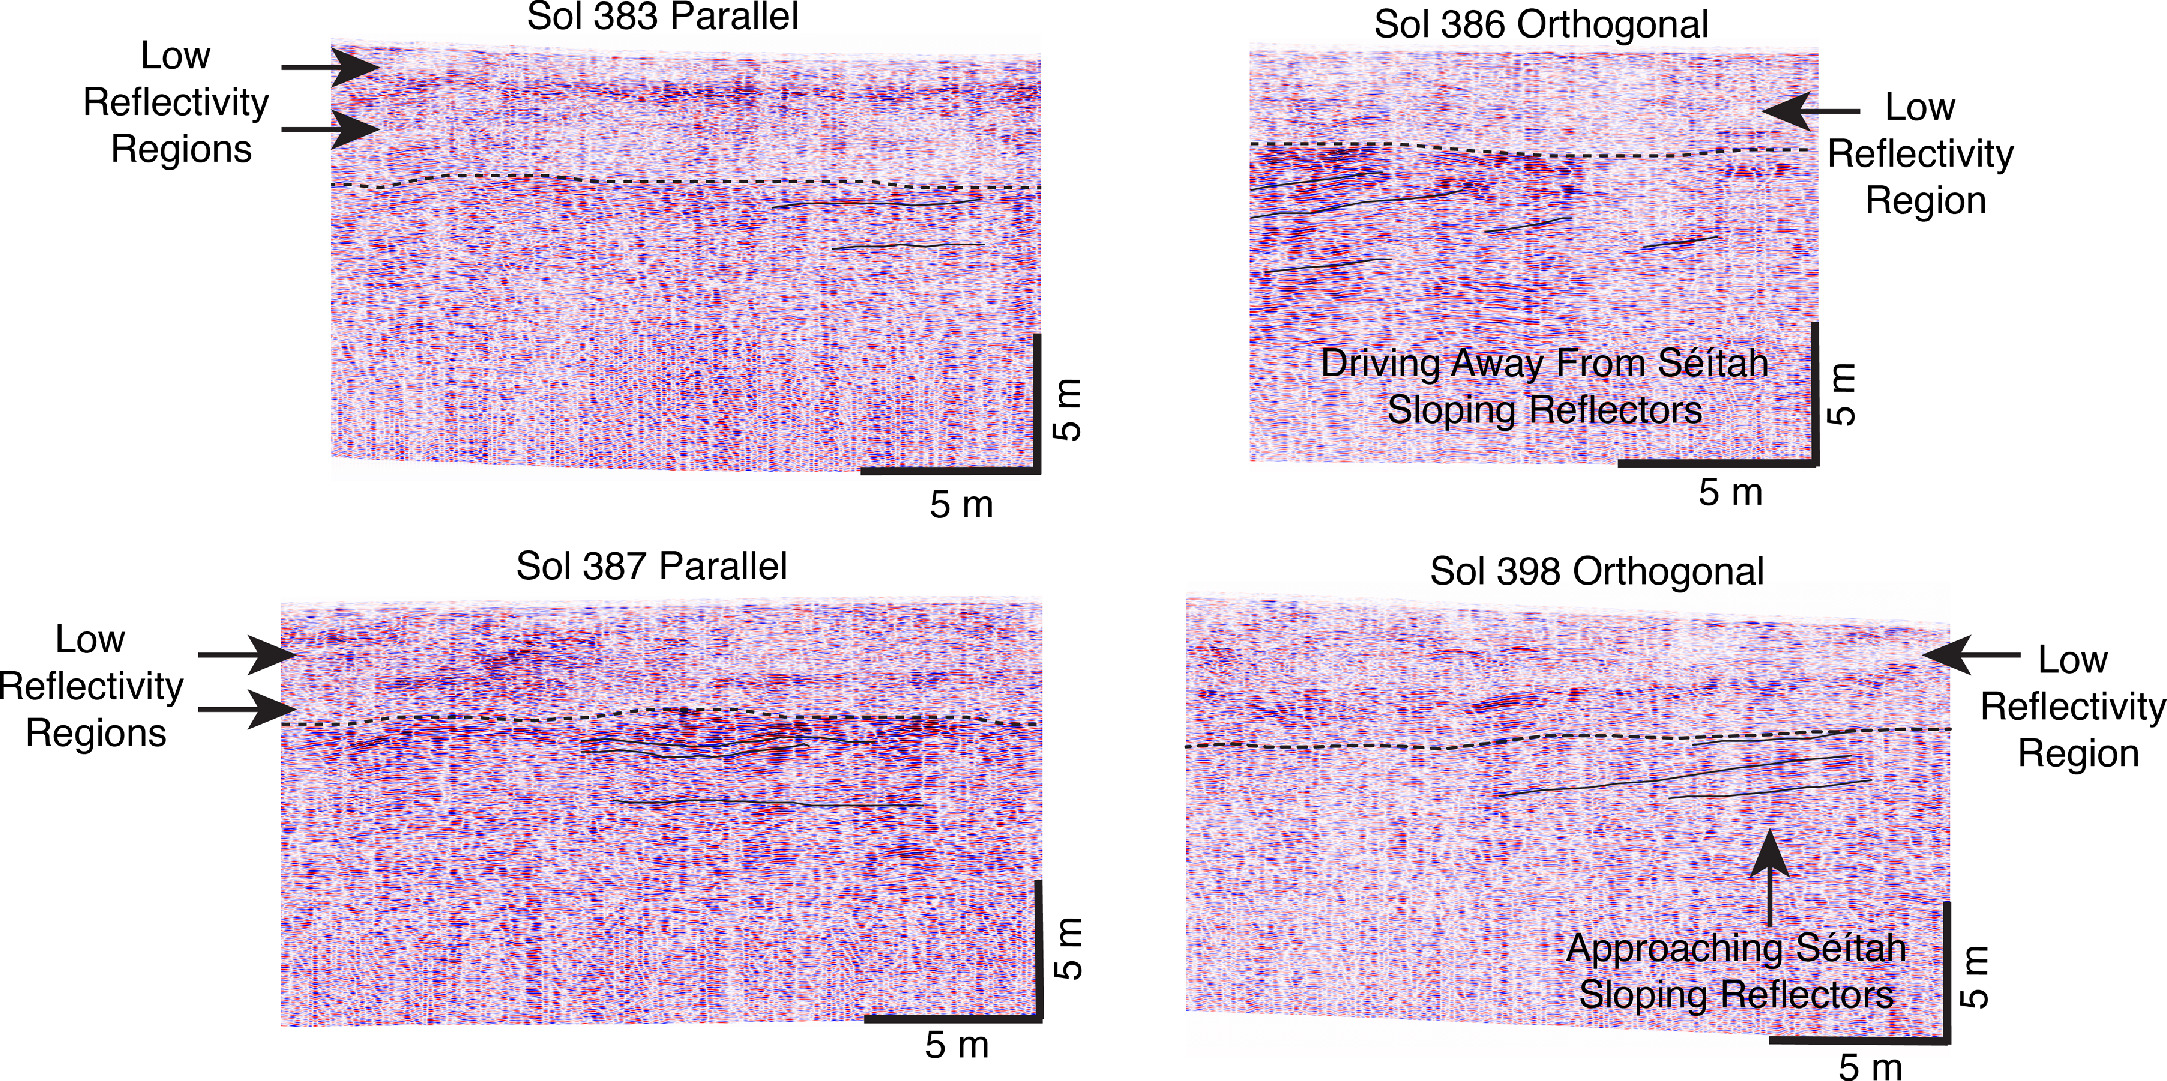
\includegraphics[width=0.9\linewidth]{Figures/0.5RIMFAX/Shoemaker_2024-f4.jpg}
    \caption[RIMFAX traverse from sols 383, 386, 387, and 398.]{RIMFAX traverse from sols 383, 386, 387, and 398 \citep{shoemaker2024}. \textbf{Keywords:} Sloping reflectors, parallel, low reflectivity, horizontal layering, multidirectional dipping.}
    \label{fig:Shoemaker24-4}
\end{figure}

\begin{figure}[h!]
    \centering
    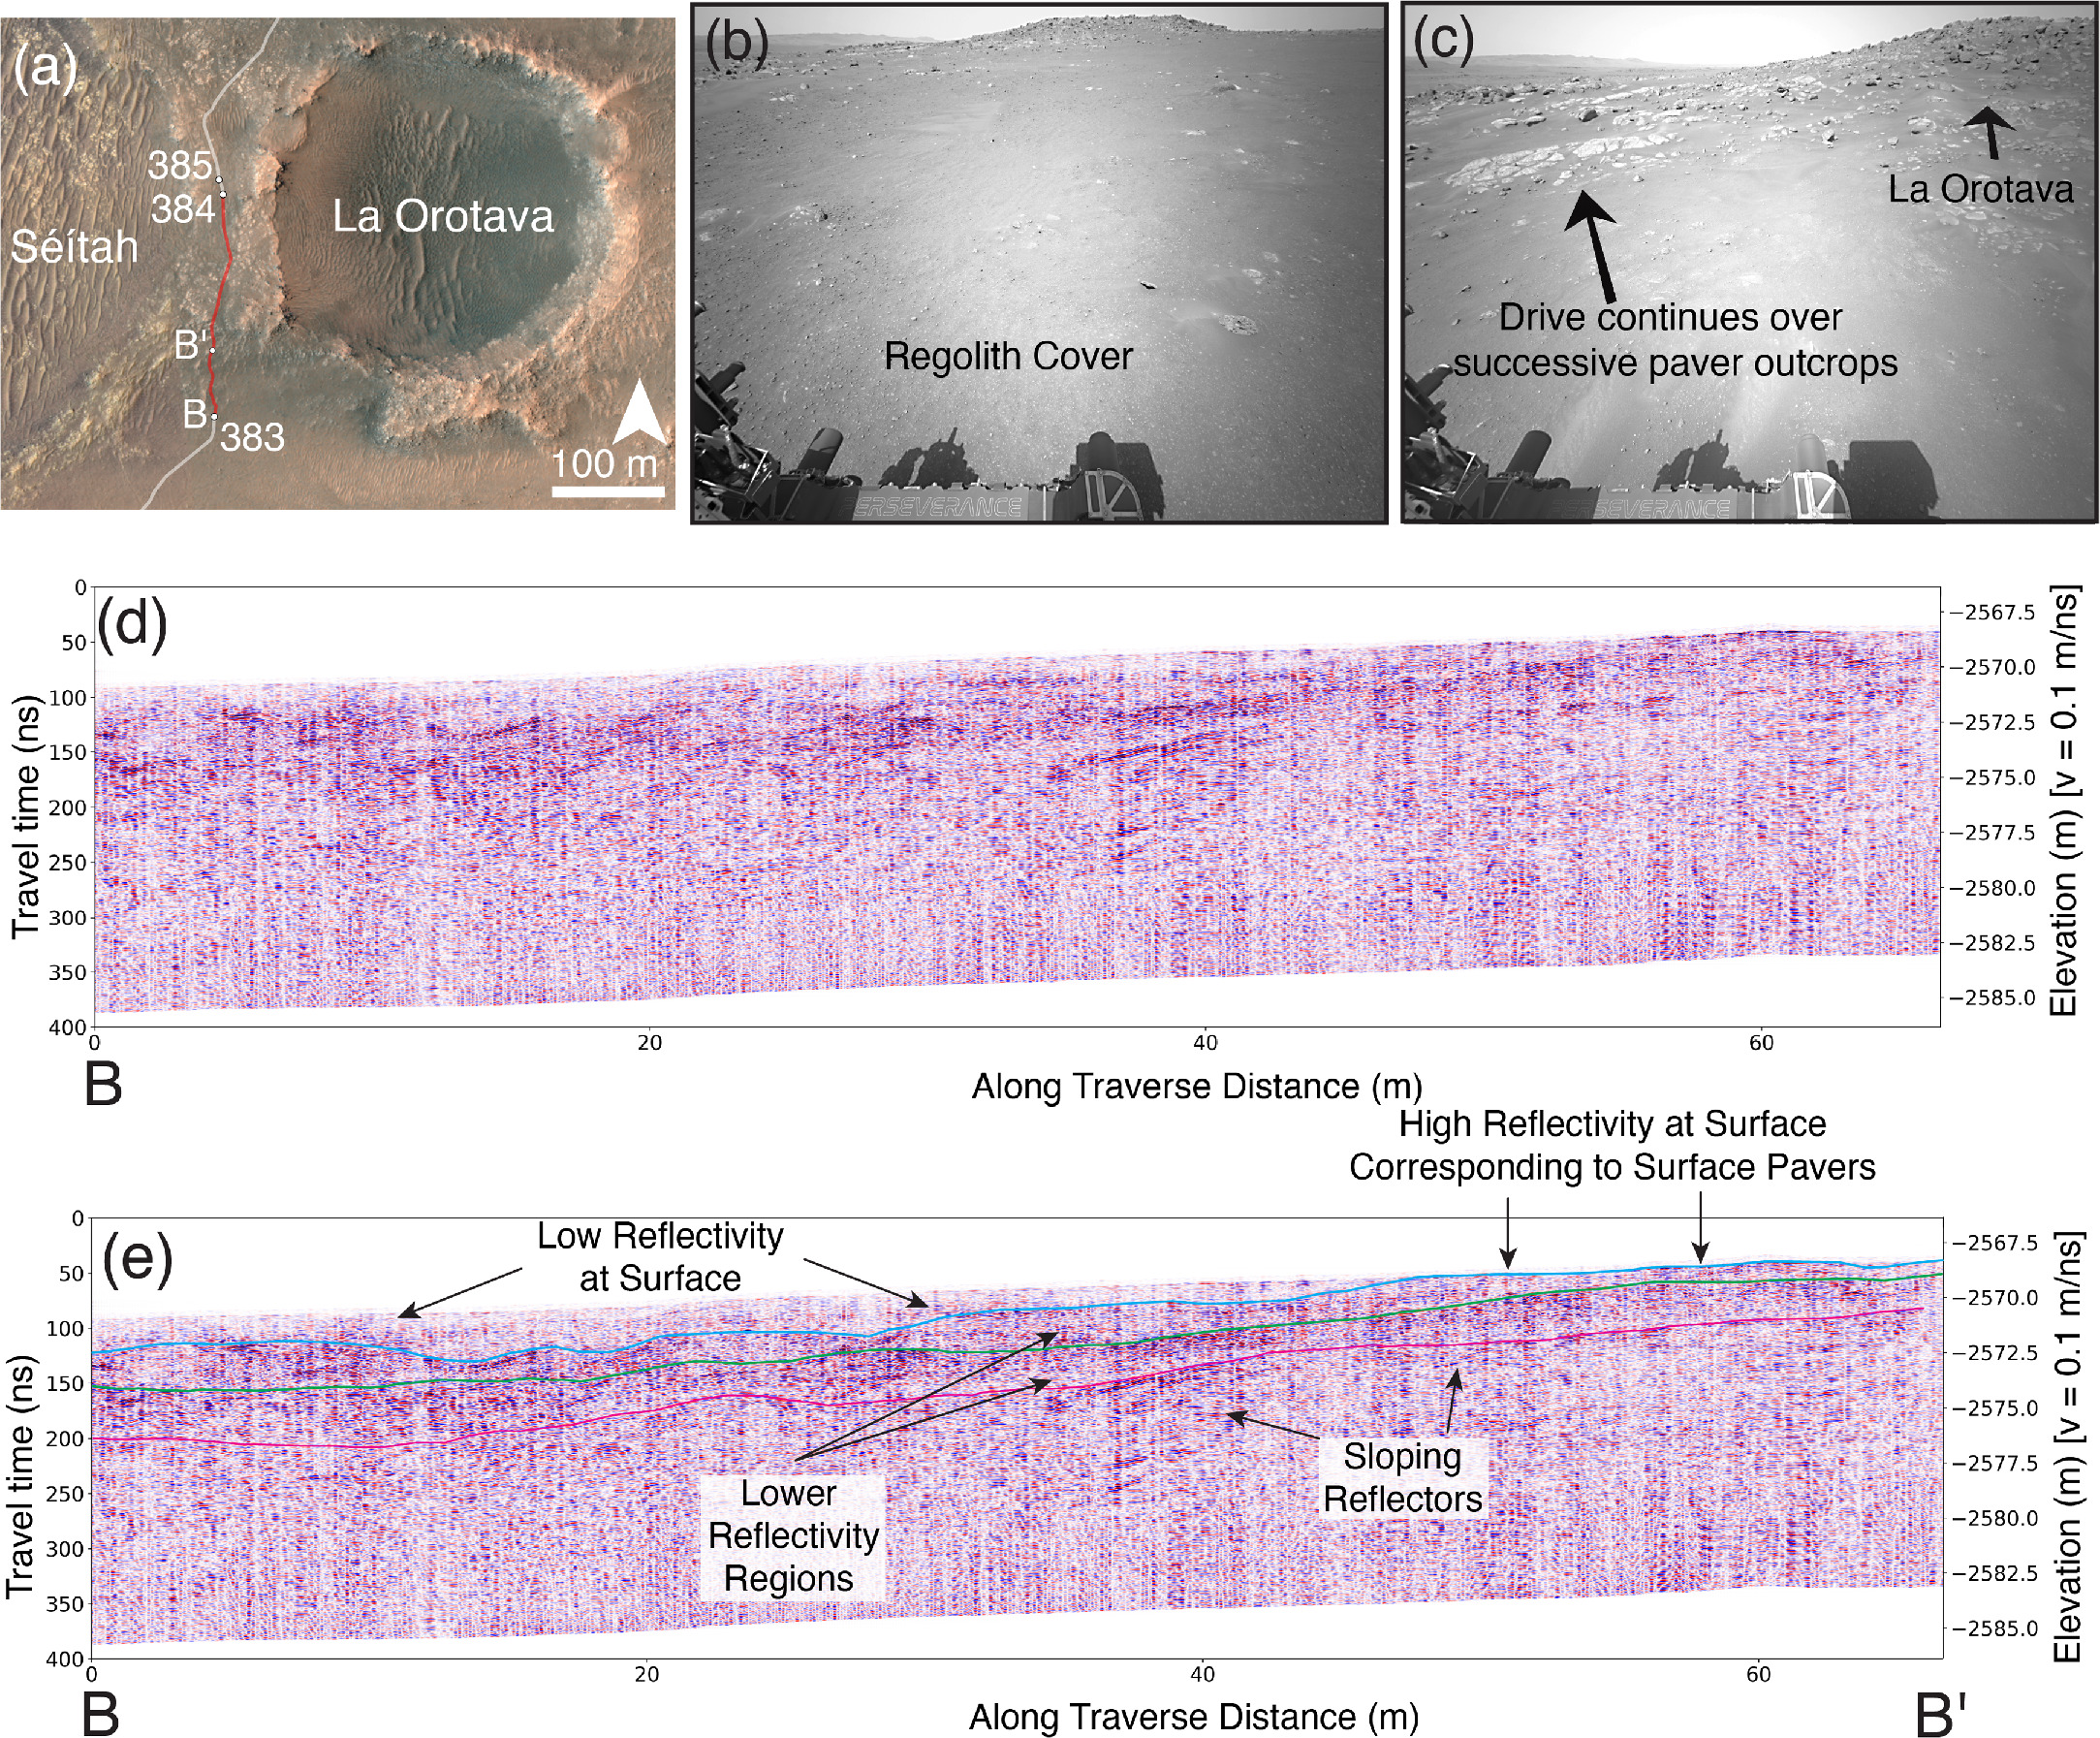
\includegraphics[width=0.9\linewidth]{Figures/0.5RIMFAX/Shoemaker_2024-f5.jpg}
    \caption[RIMFAX radargram from sol 384]{RIMFAX radargram from sol 384 \citep{shoemaker2024}. \textbf{Keywords:} Truncation, high reflectivity, low reflectivity, dipping reflectors, semi-continuous, sloping reflectors.}
    \label{fig:Shoemaker24-5}
\end{figure}

\begin{figure}[h!]
    \centering
    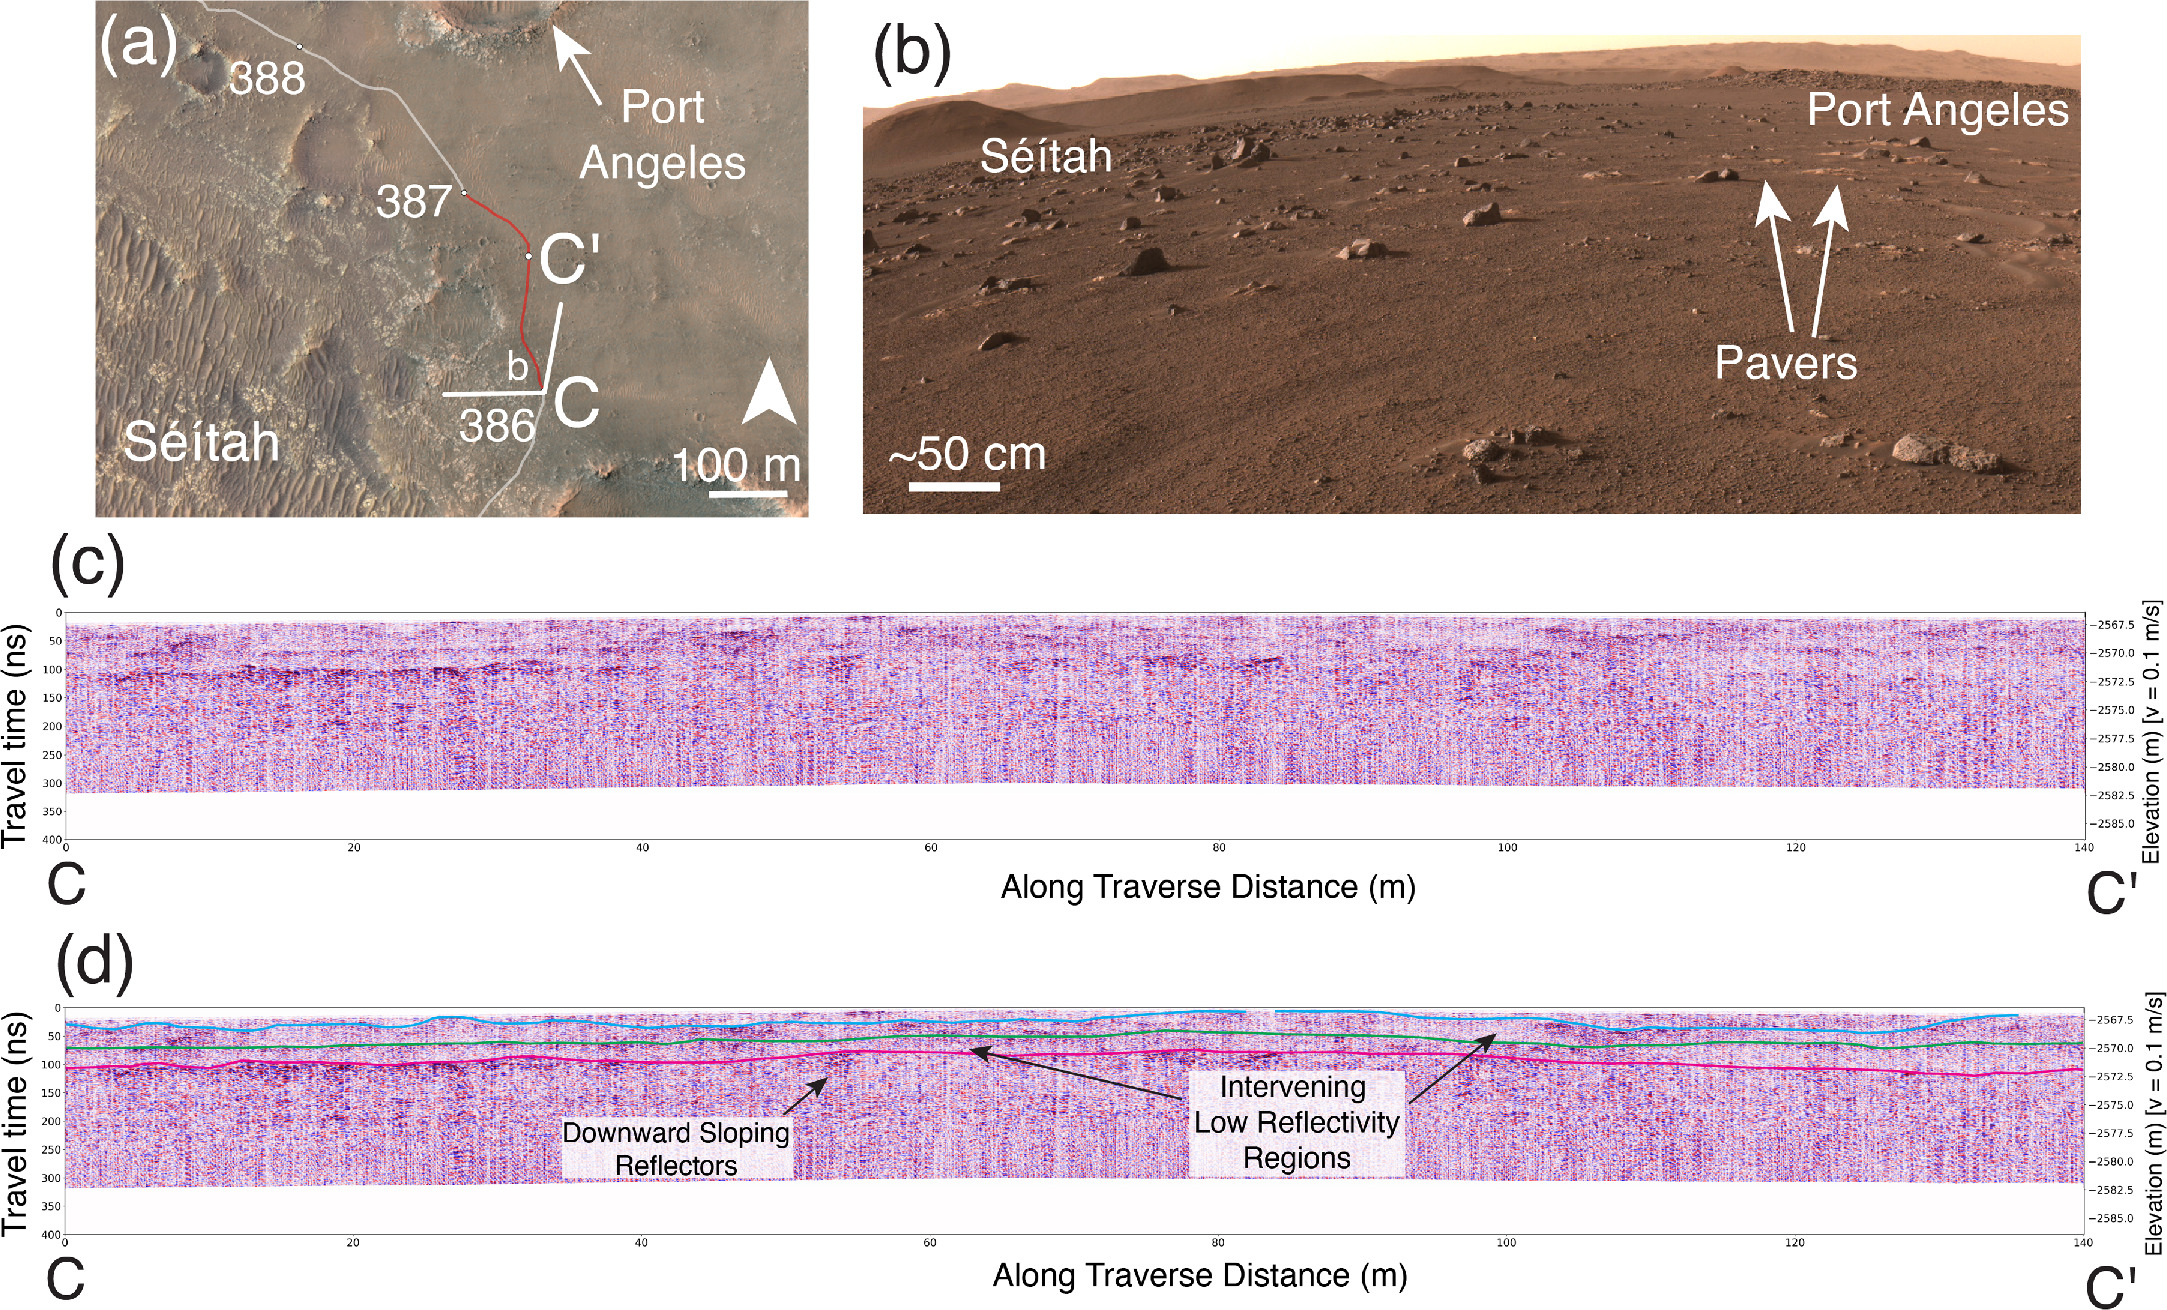
\includegraphics[width=0.9\linewidth]{Figures/0.5RIMFAX/Shoemaker_2024-f8.jpg}
    \caption[RIMFAX radargram from sol 387.]{RIMFAX radargram from sol 387 \citep{shoemaker2024}. \textbf{Keywords:} Sloping reflectors, semi-continuous layering, parallel, semi-horizontal layering, low reflectivity, high reflectivity.}
    \label{fig:Shoemaker24-8}
\end{figure}

\begin{figure}[h!]
    \centering
    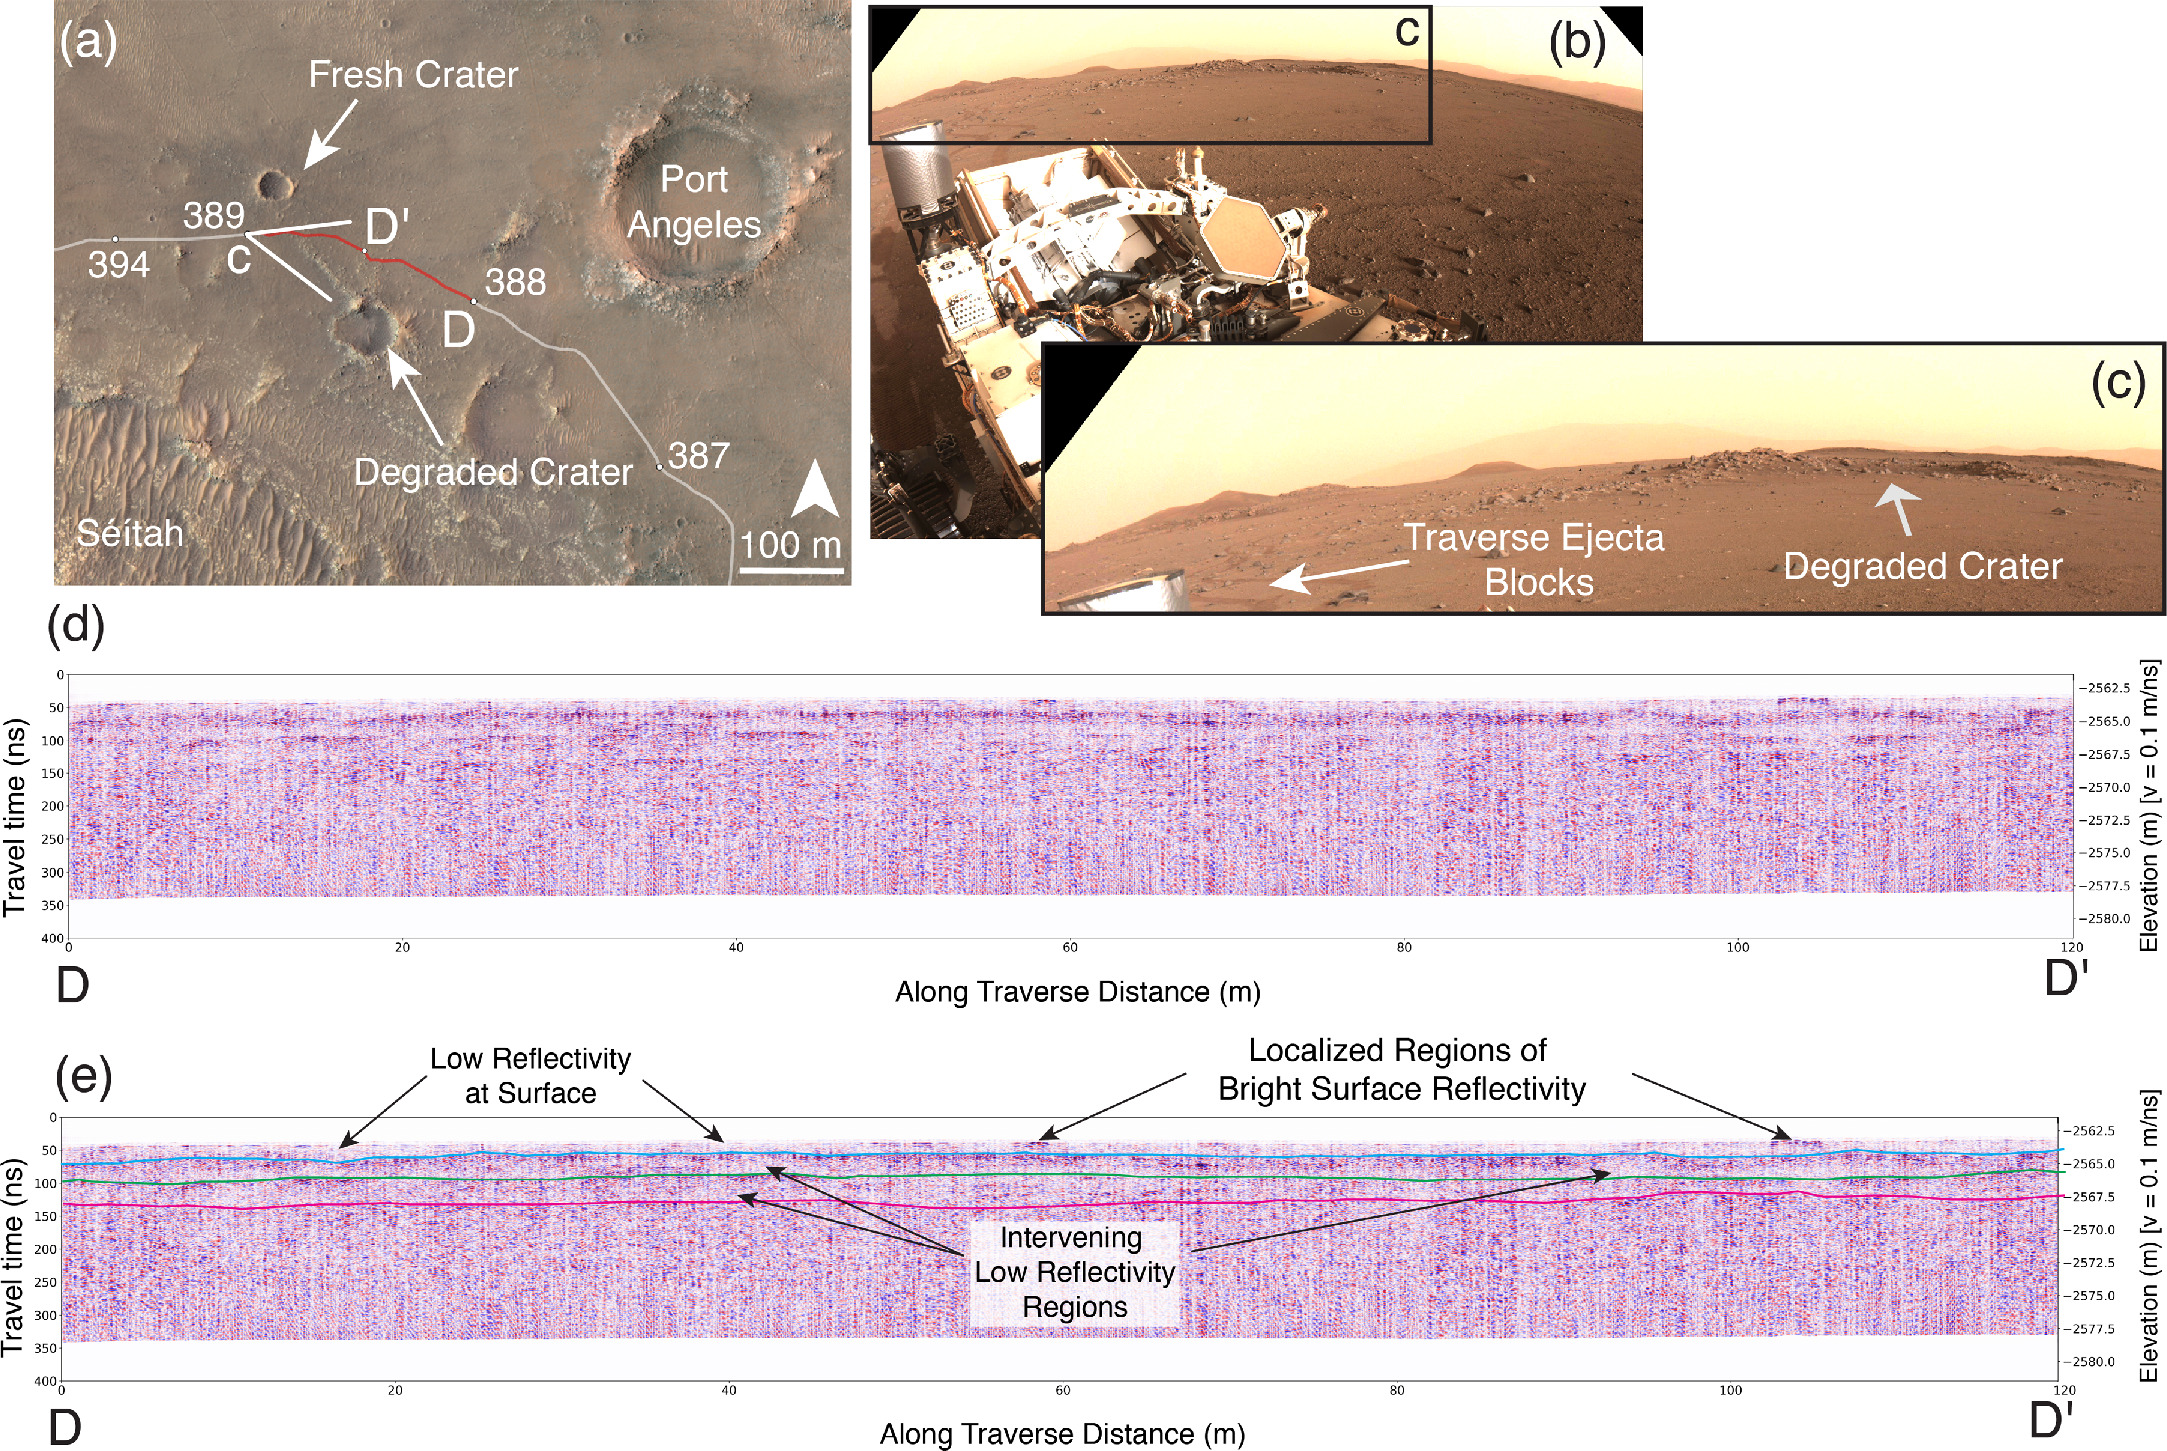
\includegraphics[width=0.9\linewidth]{Figures/0.5RIMFAX/Shoemaker_2024-f10.jpg}
    \caption[RIMFAX traverse from sol 389]{RIMFAX traverse from sol 389 \citep{shoemaker2024}. \textbf{Keywords:} Parallel, high reflectivity, low reflectivity, semi-continuous, sloping reflectors.}
    \label{fig:Shoemaker24-10}
\end{figure}

\begin{figure}[h!]
    \centering
    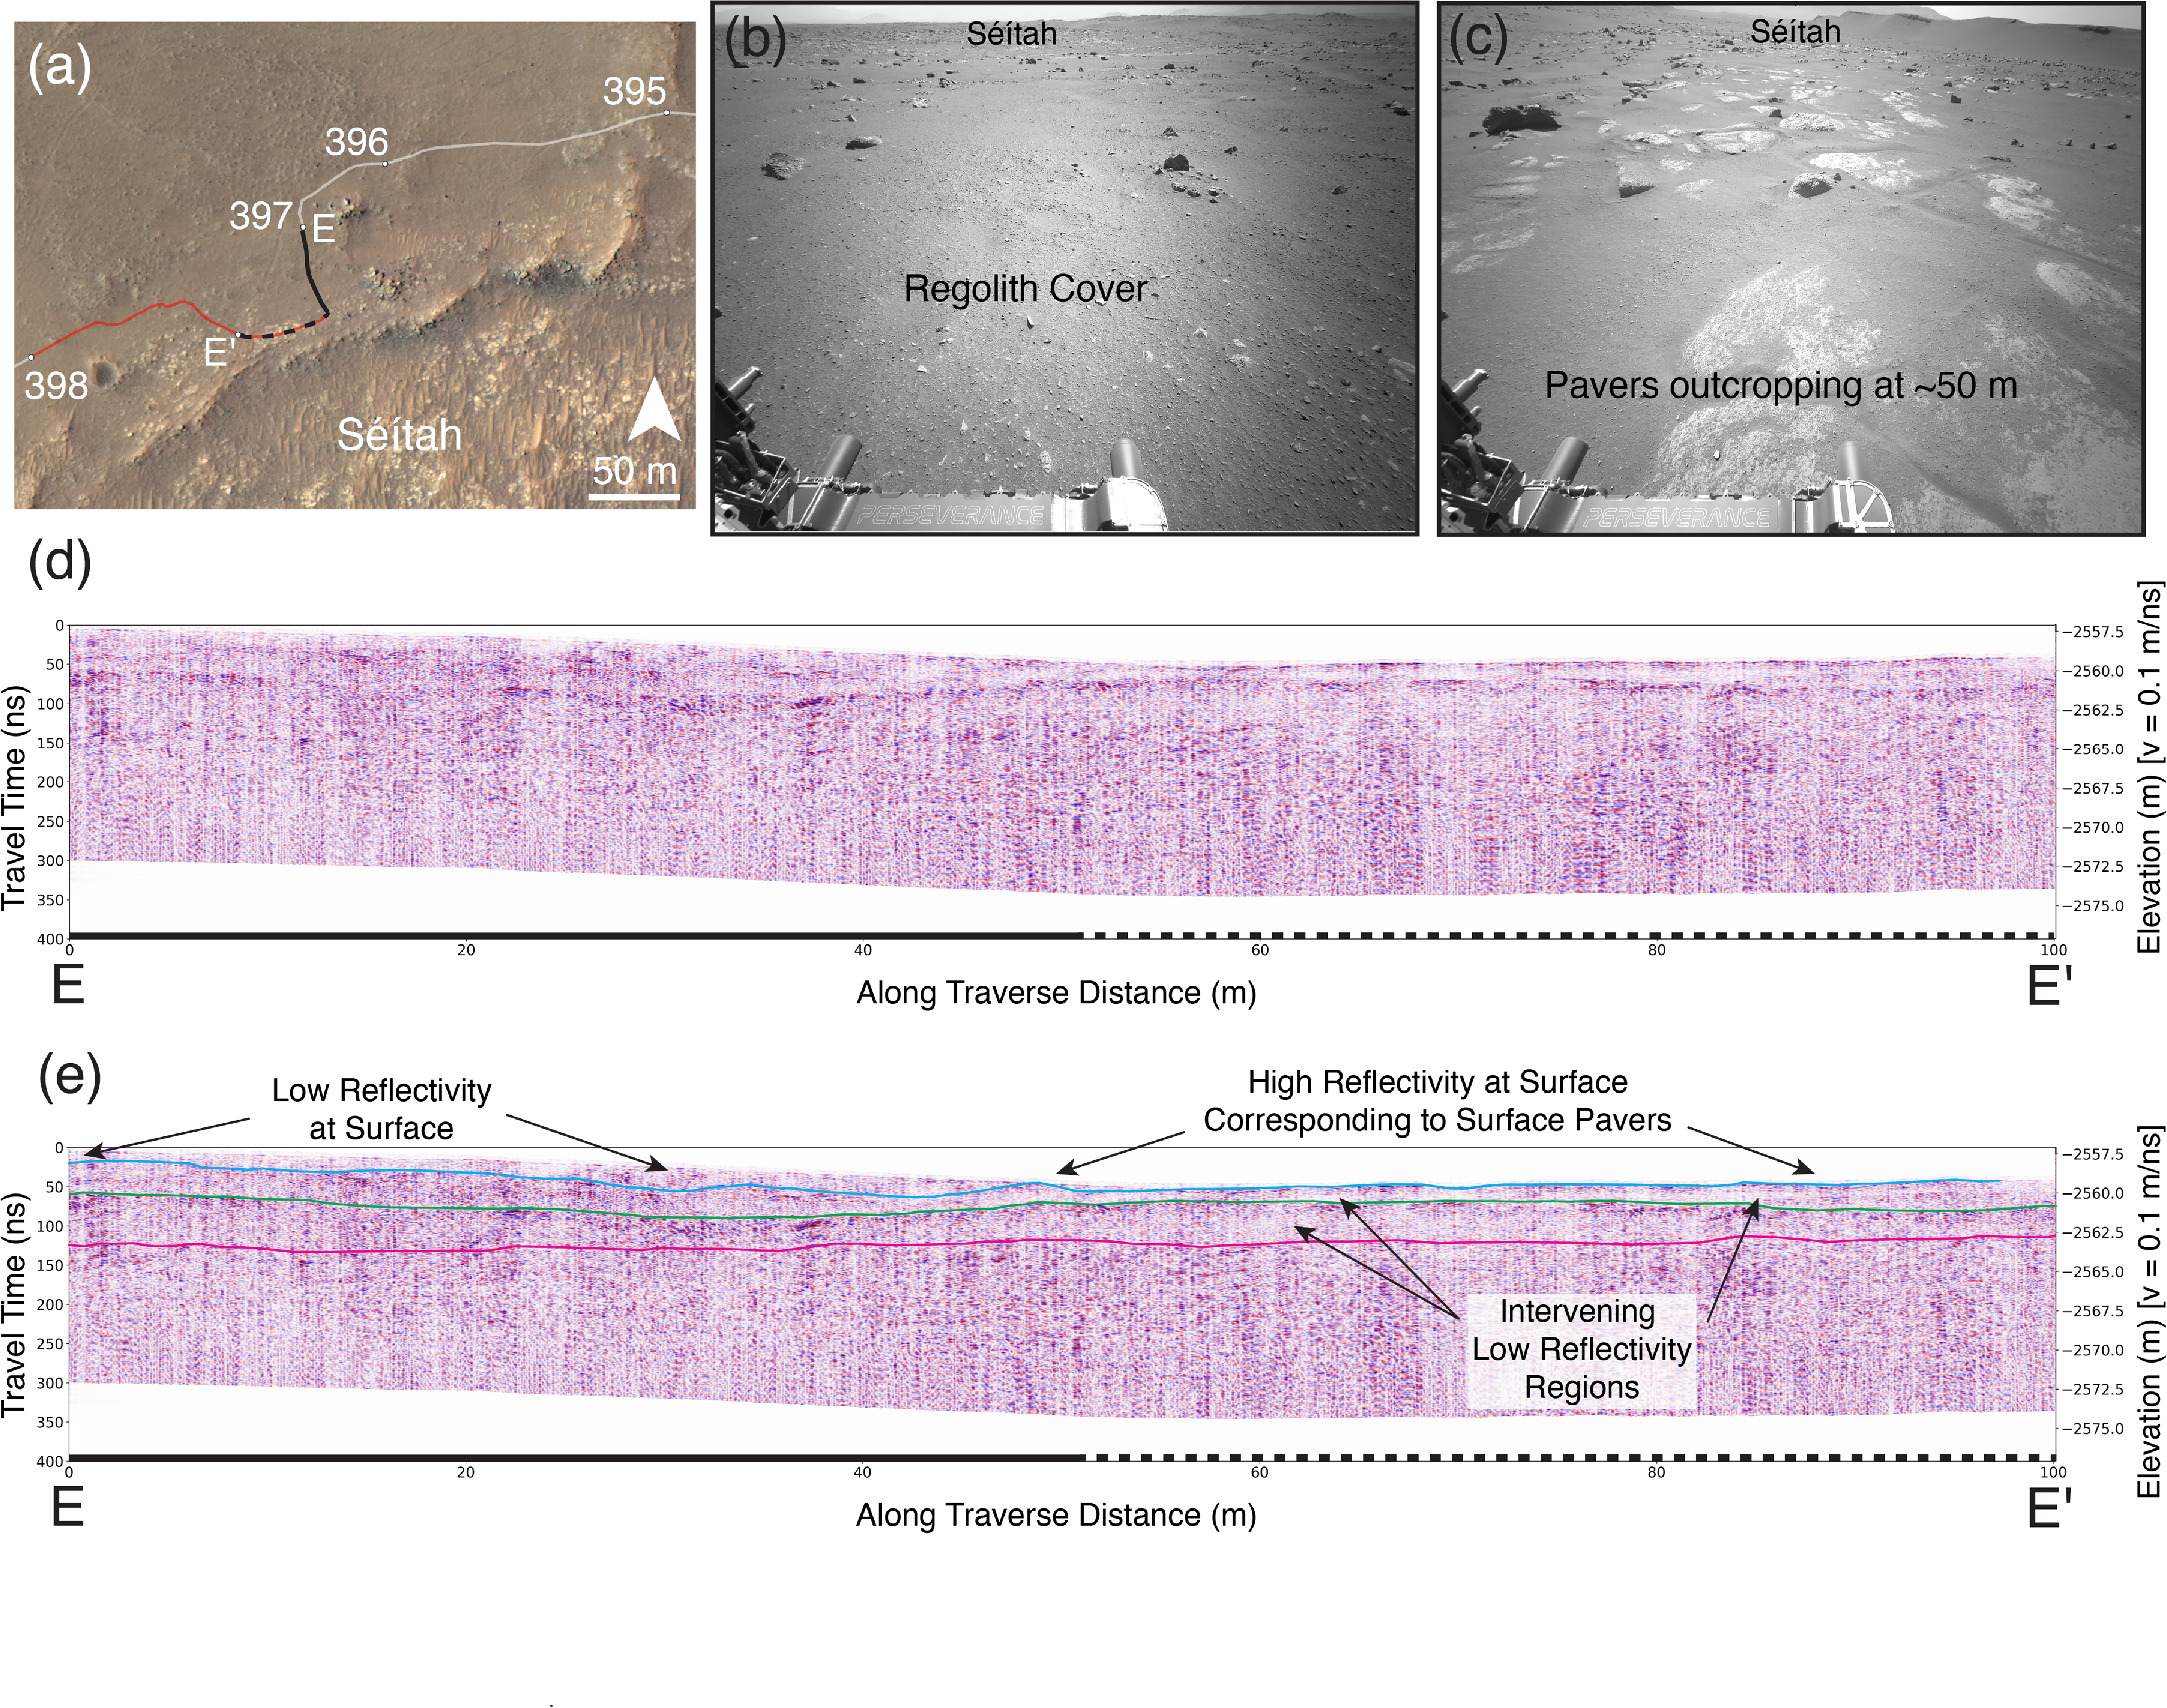
\includegraphics[width=0.9\linewidth]{Figures/0.5RIMFAX/Shoemaker_2024-f12.jpg}
    \caption[RIMFAX traverse sol 398.]{RIMFAX traverse sol 398 \citep{shoemaker2024}.\textbf{Keywords:} Parallel, high reflectivity, low reflectivity, dipping reflectors, semi-continuous, sloping reflectors.}
    \label{fig:Shoemaker24-12}
\end{figure}

\begin{figure}[h!]
    \centering
    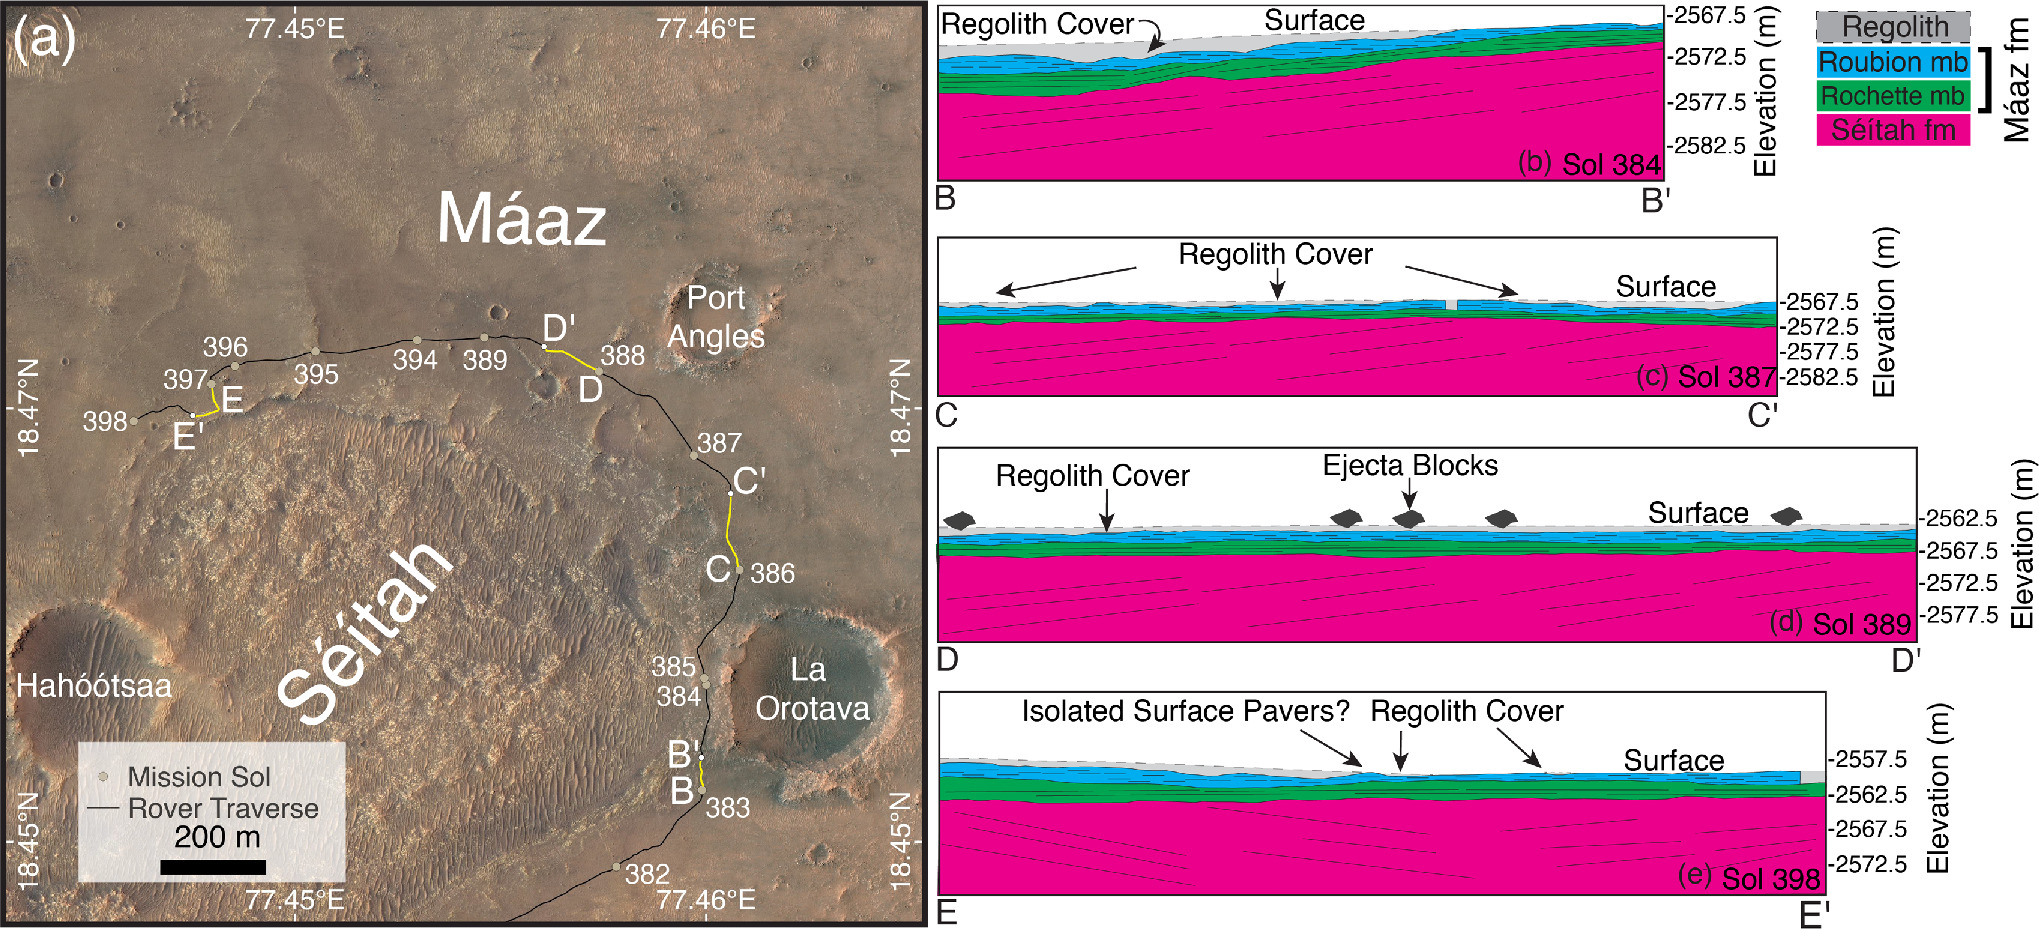
\includegraphics[width=0.9\linewidth]{Figures/0.5RIMFAX/Shoemaker_2024-f16.jpg}
    \caption[RIMFAX radargrams images on sols 384, 387, 389, and 398.]{RIMFAX radargrams images on sols 384, 387, 389, and 398 \citep{shoemaker2024}. \textbf{Keywords:} Horizontal layering, dipping reflectors, multi-directional dipping.} 
    \label{fig:Shoemaker24-16}
\end{figure}
\clearpage
\subsubsection{Lacustrine delta deposits}
\begin{figure}[h!]
    \centering
    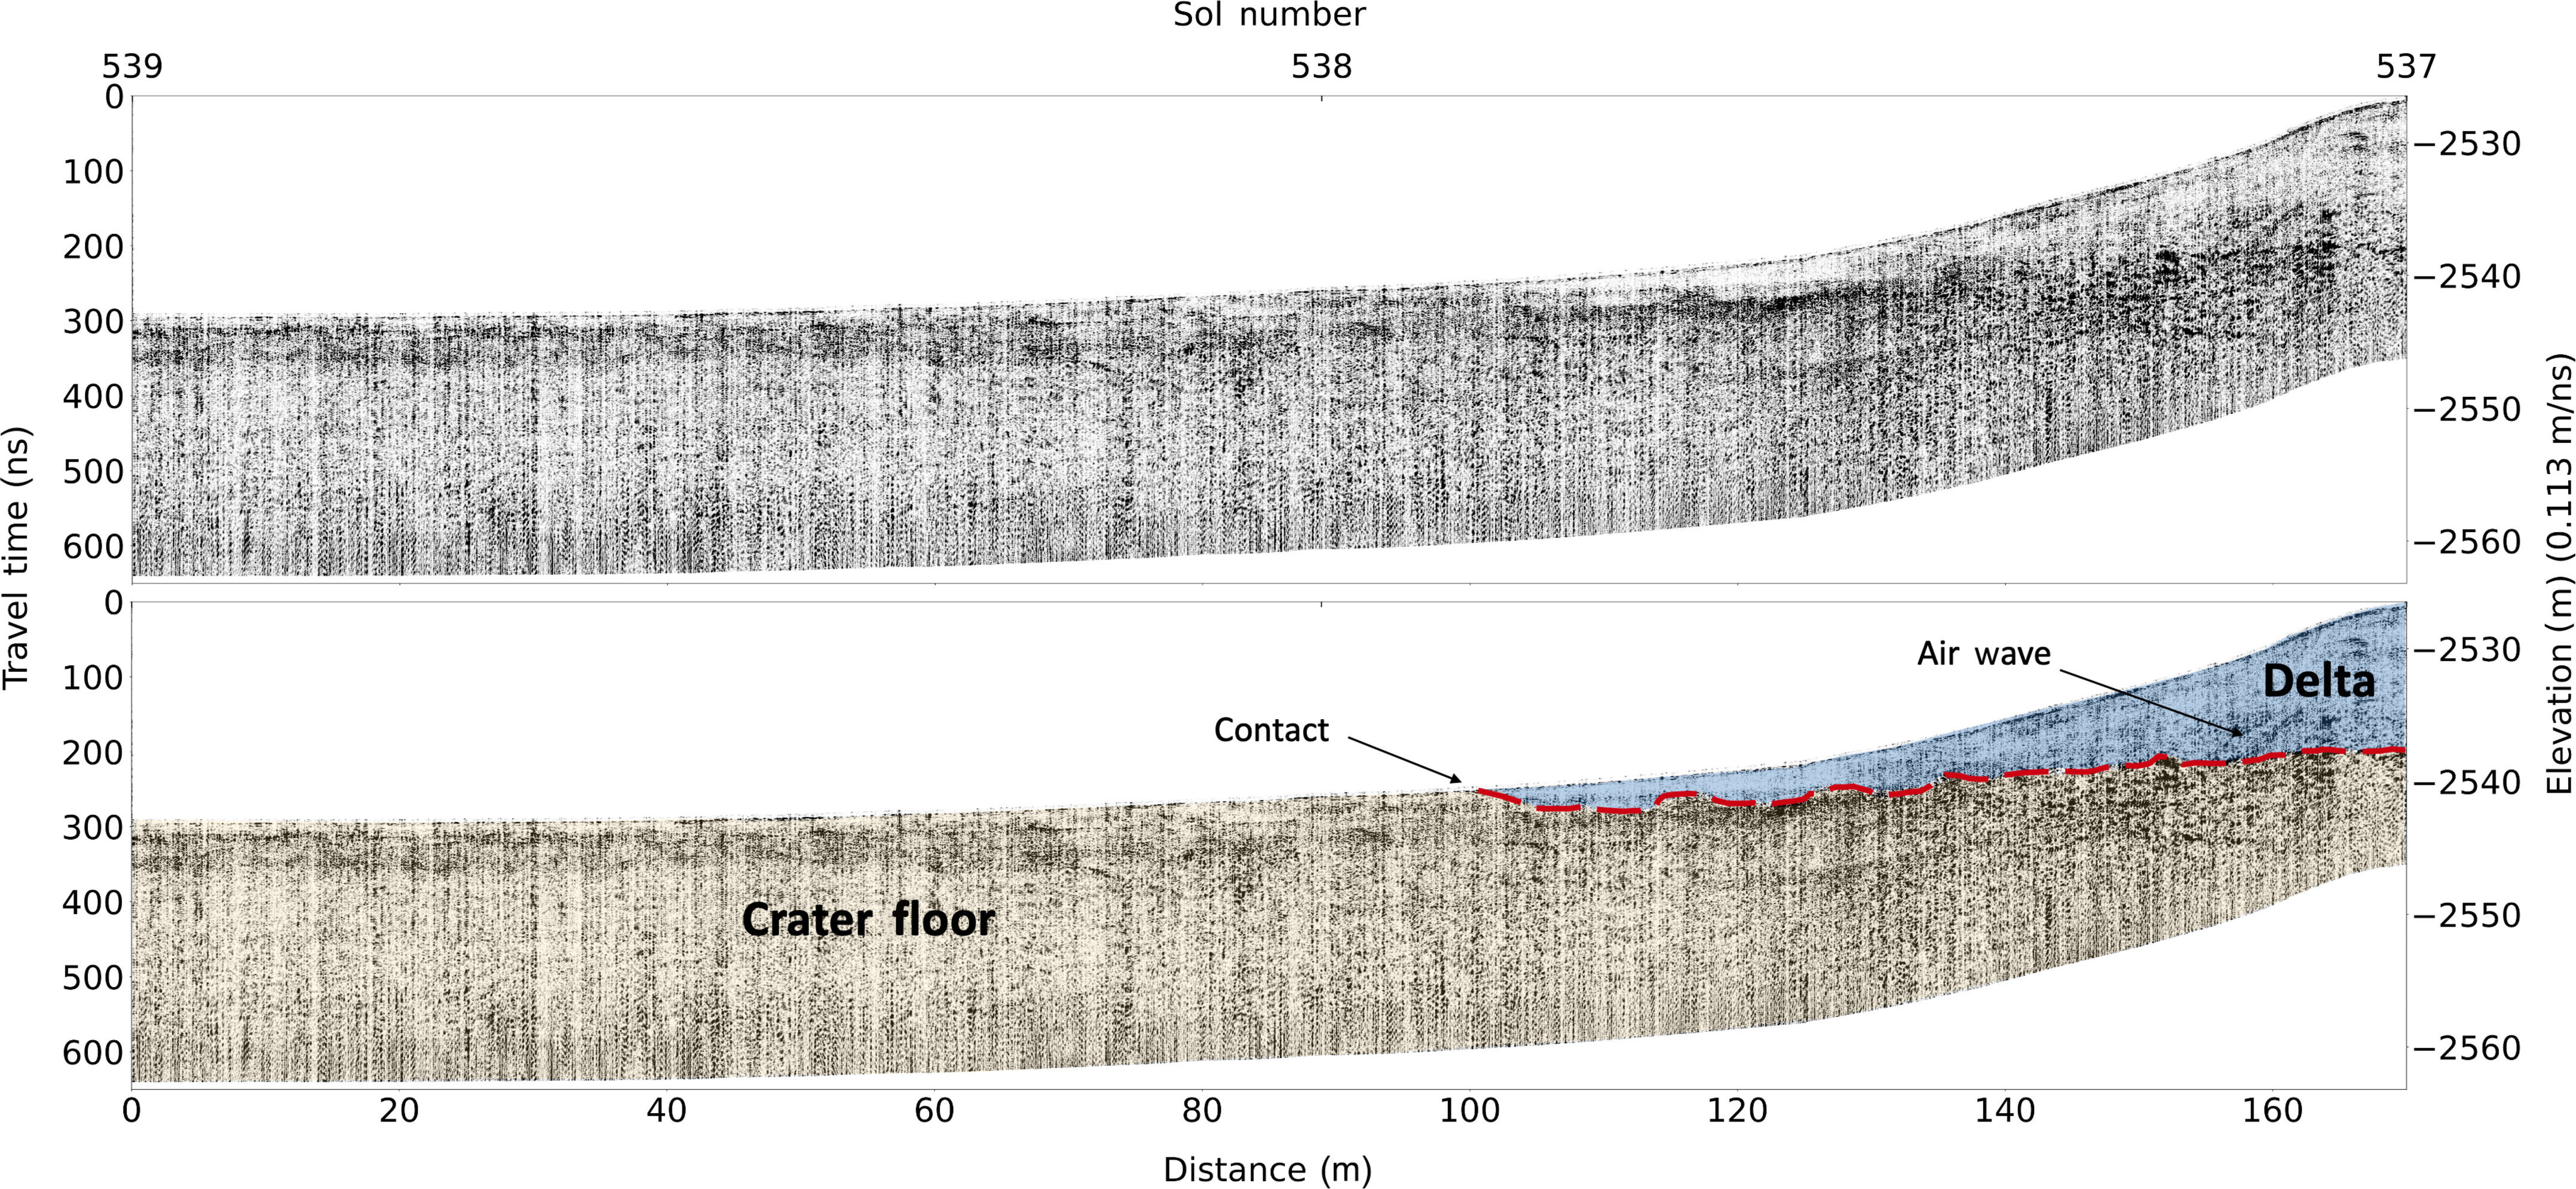
\includegraphics[width=0.9\linewidth]{Figures/0.5RIMFAX/Paige_2024-f3.jpg}
    \caption[RIMFAX traverse from sol 538–539]{RIMFAX traverse from sol 538–539 \citep{Paige2024}. \textbf{Keywords:} Erosional contact, multi-directional dipping, semi-continuous layers, high reflectivity, low reflectivity.}
    \label{fig:Paige24-3}
\end{figure}

\begin{figure}[h!]
    \centering
    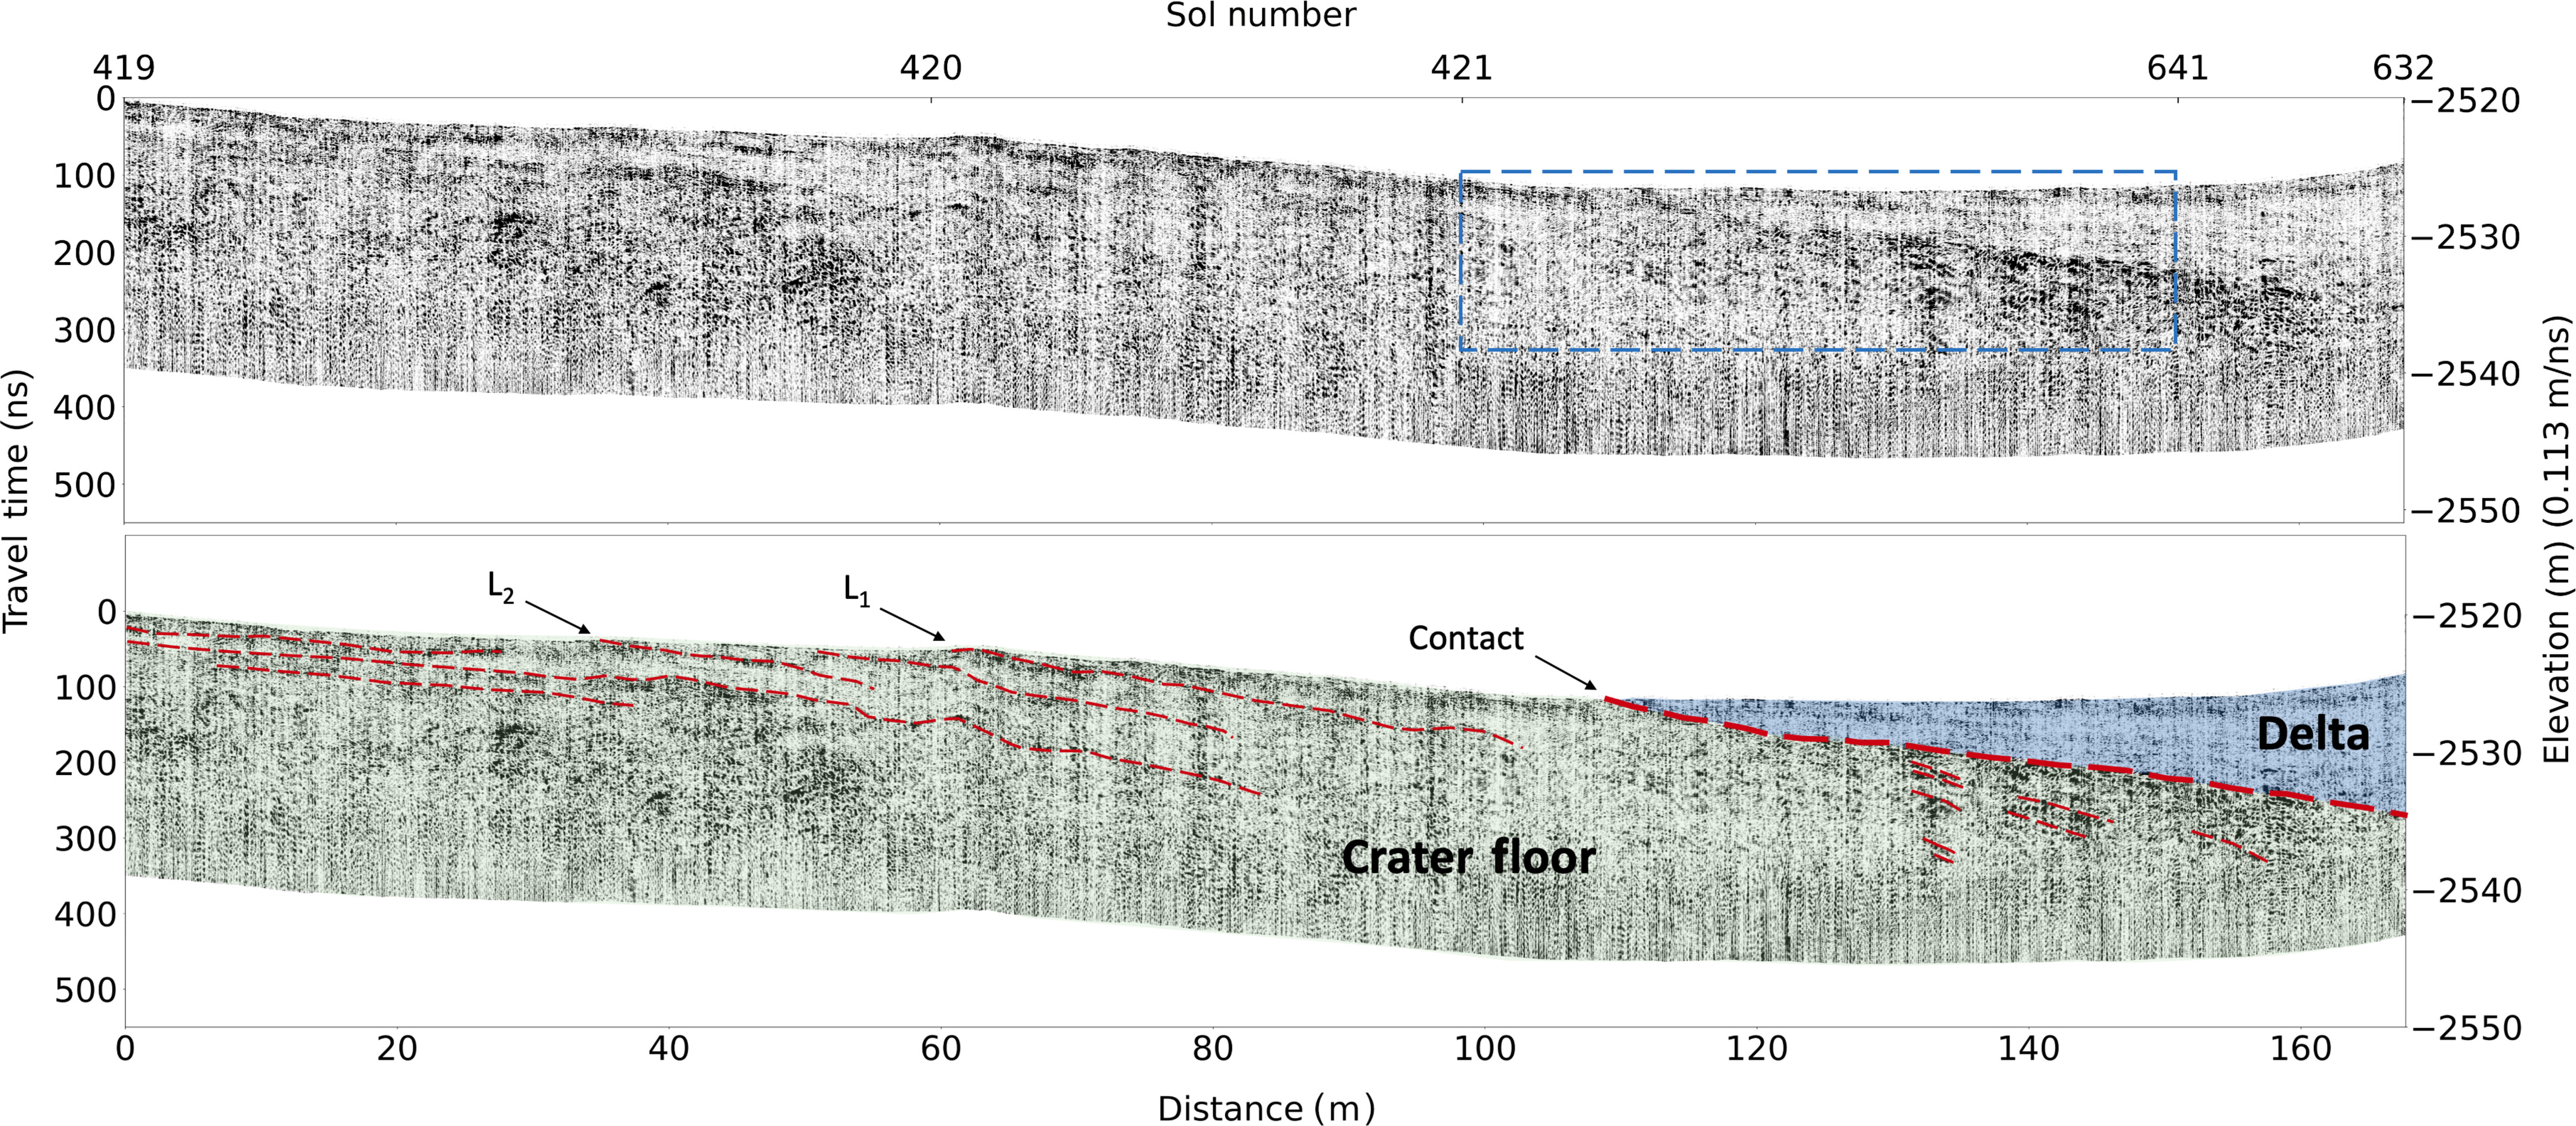
\includegraphics[width=0.9\linewidth]{Figures/0.5RIMFAX/Paige_2024-f4.jpg}
    \caption[RIMFAX observed contact between the crater floor and the delta at Cape Nukshak. Sol 420–422]{RIMFAX observed contact between the crater floor and the delta at Cape Nukshak. Sol 420–422 \citep{Paige2024}.\textbf{ Keywords:} Erosional contact, multi-directional dipping, semi-continuous layers, high reflectivity, low reflectivity.}
    \label{fig:Paige24-4}
\end{figure}

\begin{figure}[h!]
    \centering
    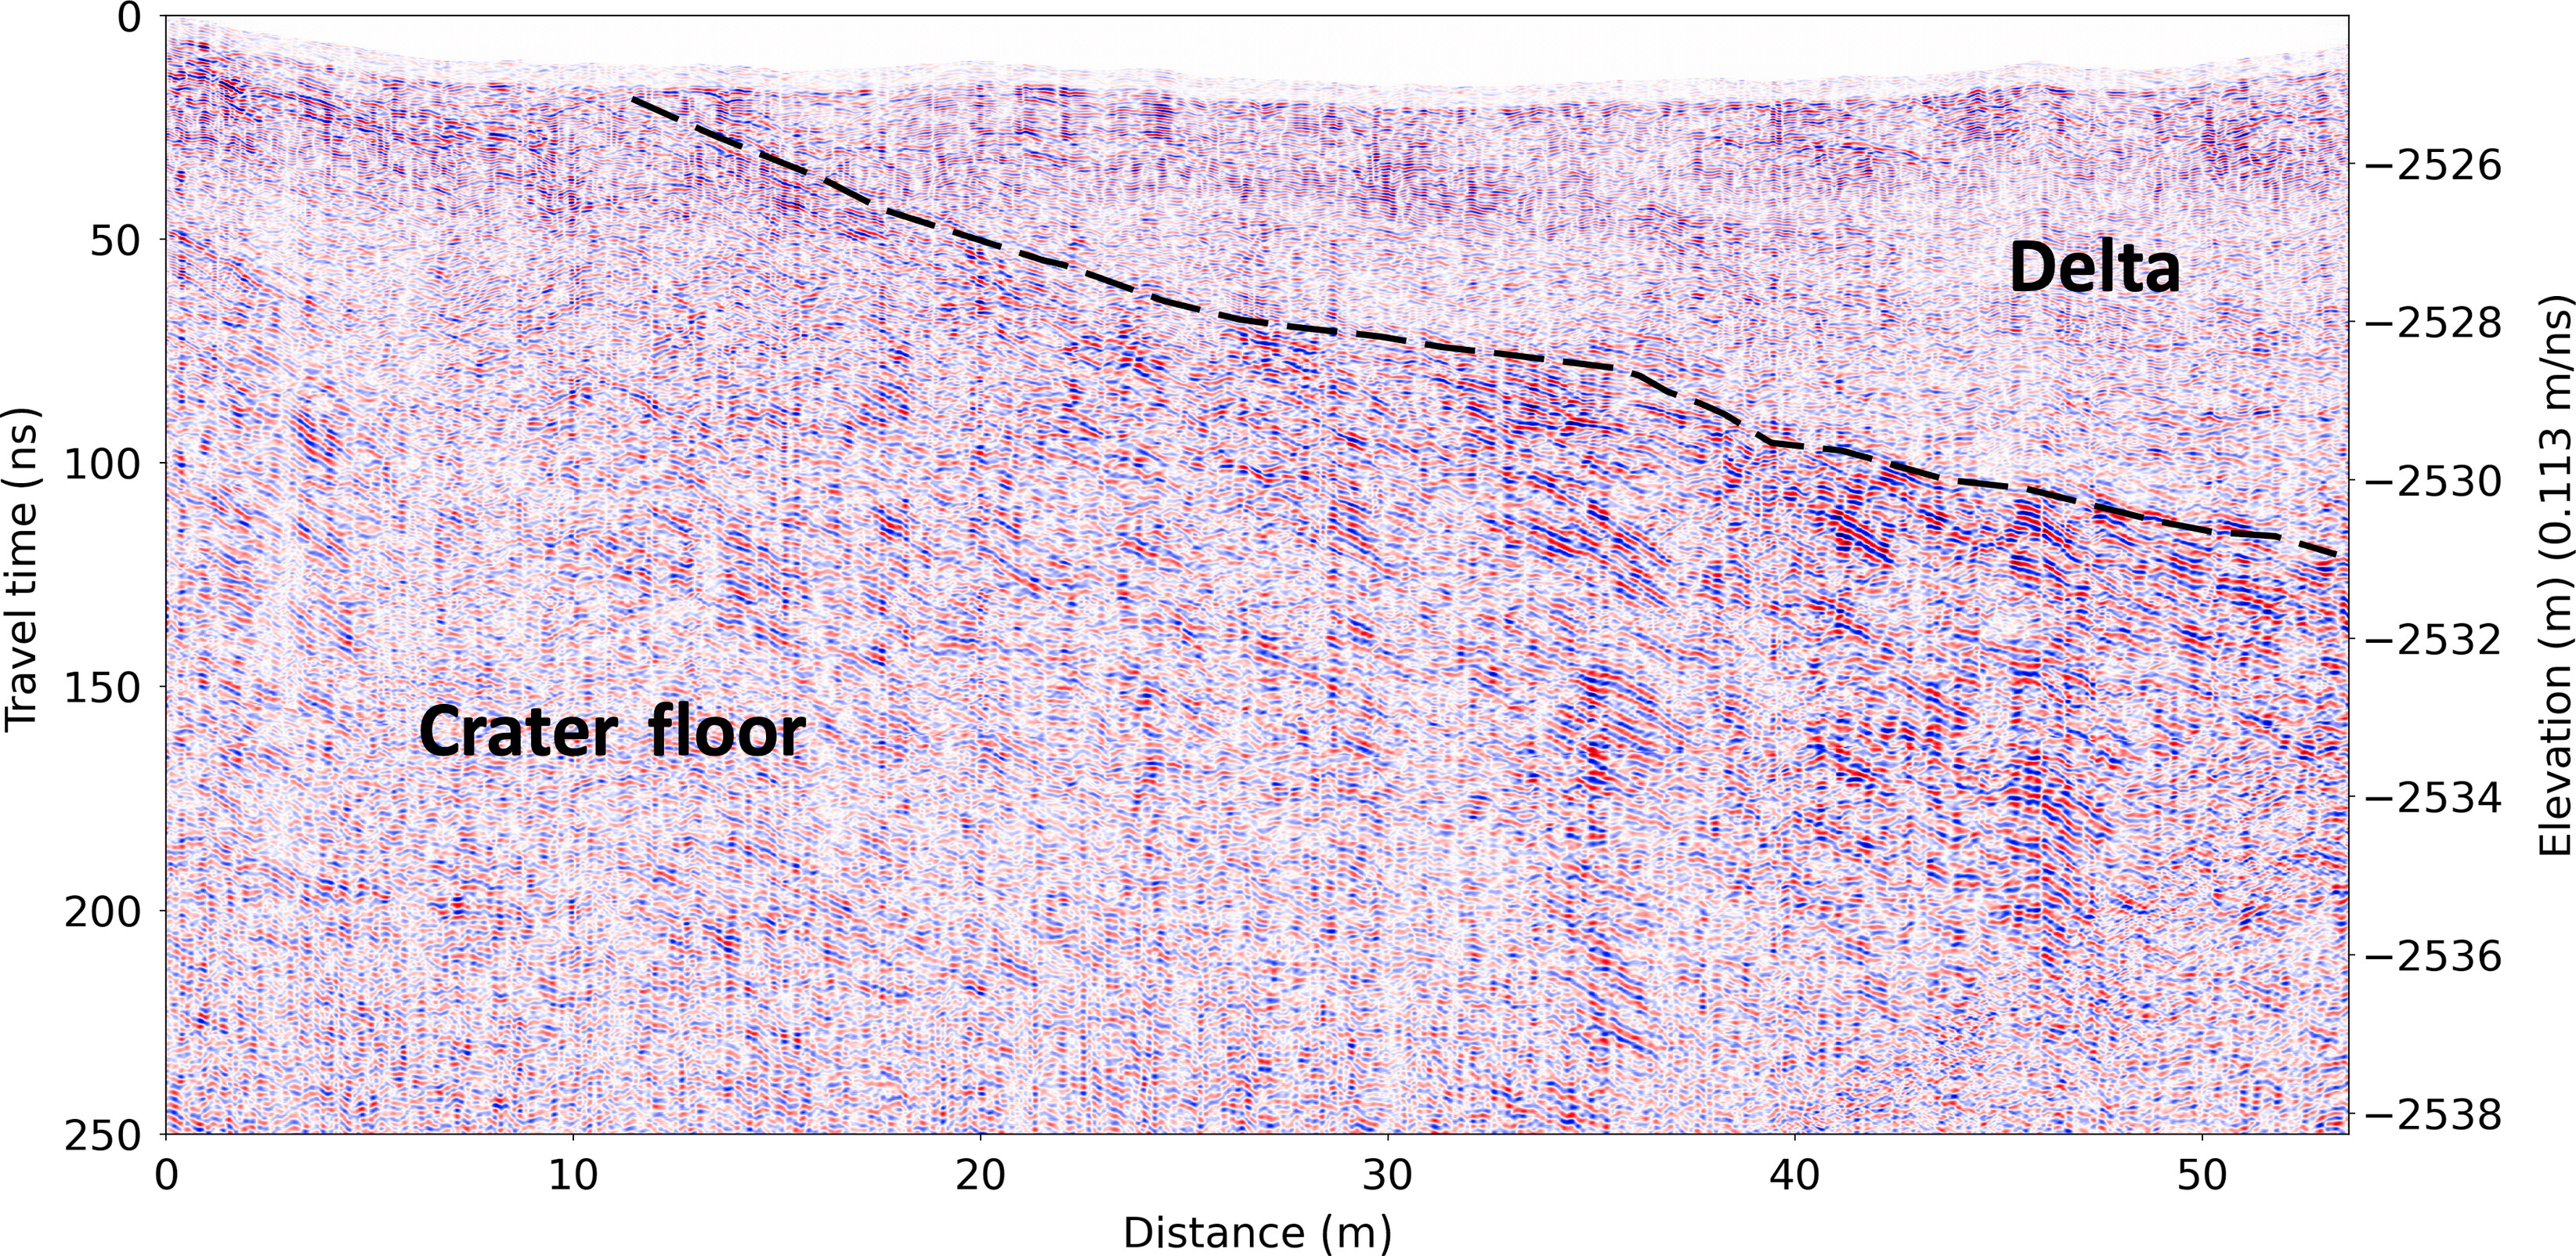
\includegraphics[width=0.9\linewidth]{Figures/0.5RIMFAX/Paige_2024-f5.jpg}
    \caption[RIMFAX radargram from sol 641]{RIMFAX radargram at Cape Nukshak from sol 641 \citep{Paige2024}. \textbf{Keywords:} Bumpy, strong reflectivity, weak reføectivity, multi-directional dipping.}
    \label{fig:Paige24-5}
\end{figure}

\begin{figure}[h!]
    \centering
    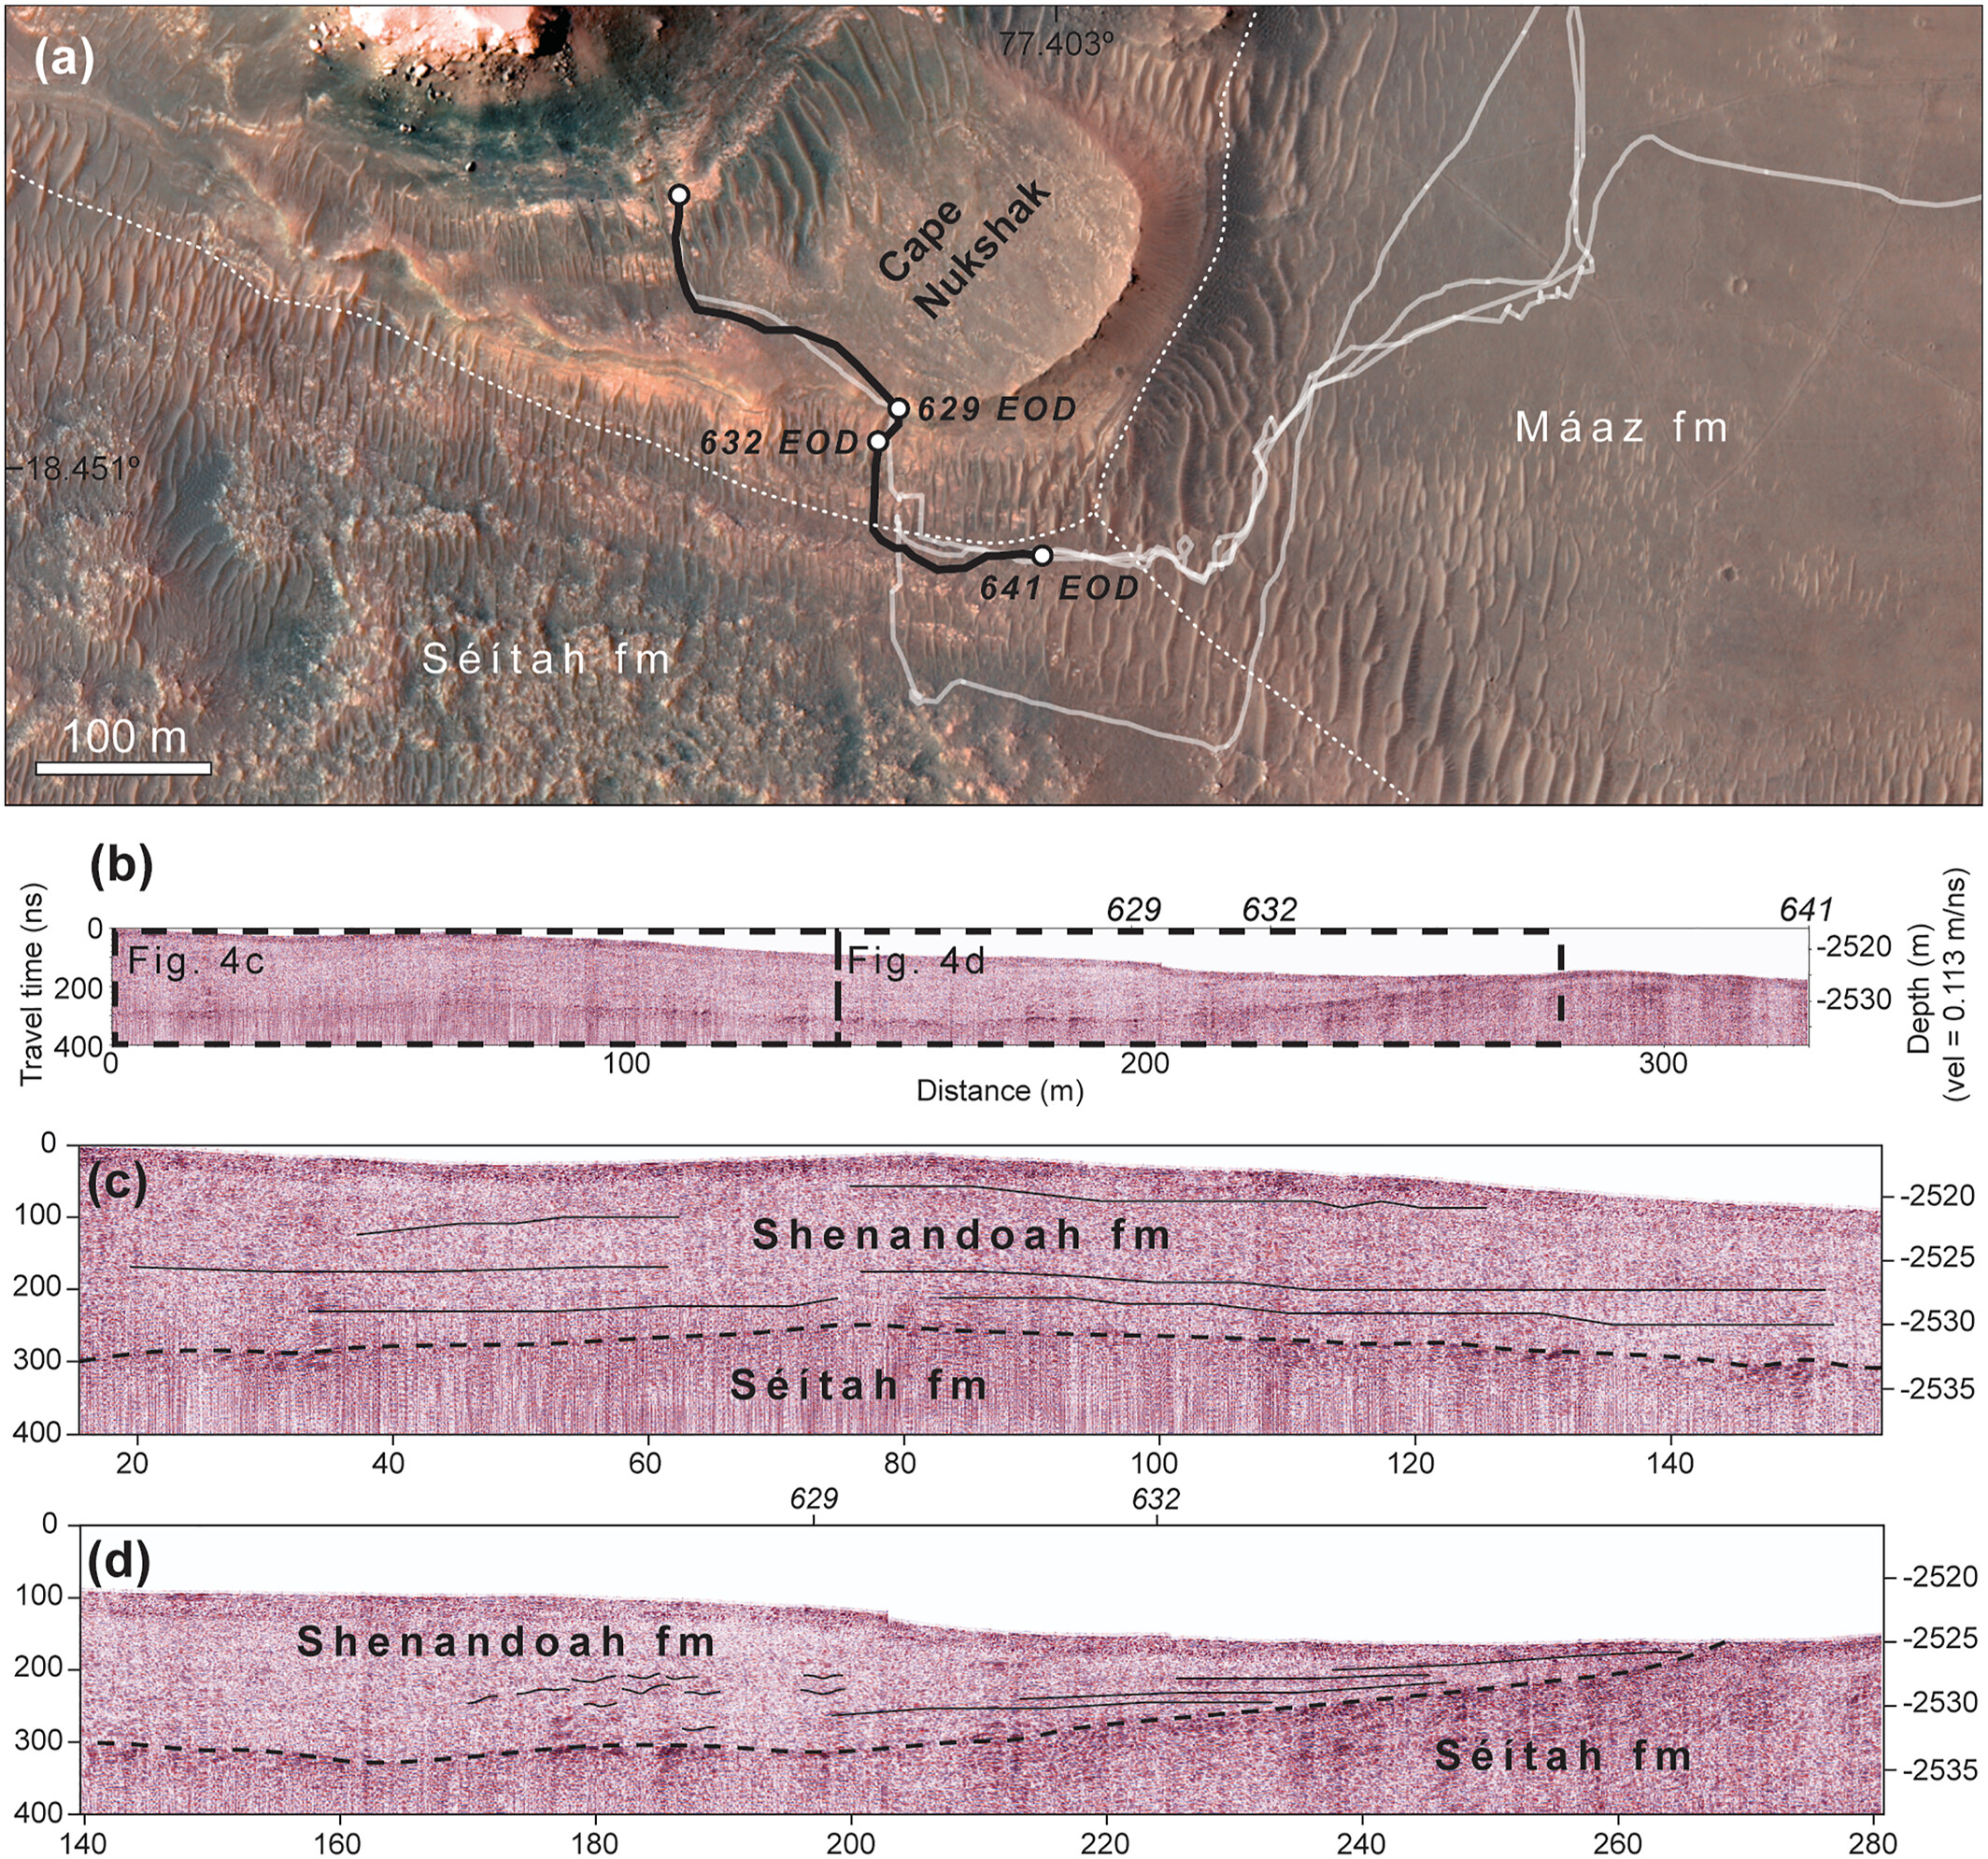
\includegraphics[width=0.9\linewidth]{Figures/0.5RIMFAX/Stack_2024-04.jpg}
    \caption[RIMFAX radargram from sols 629, 632, and 641.]{RIMFAX radargram from sols 629, 632, and 641. \textbf{Keywords:} horizontal strata, erosional contact, onlap, dipping, concave up structures, continuous, semi-continuous, low reflectivity, high-reflectivity.}
    \label{fig:Stack24-4}
\end{figure}

\begin{figure}[h!]
    \centering
    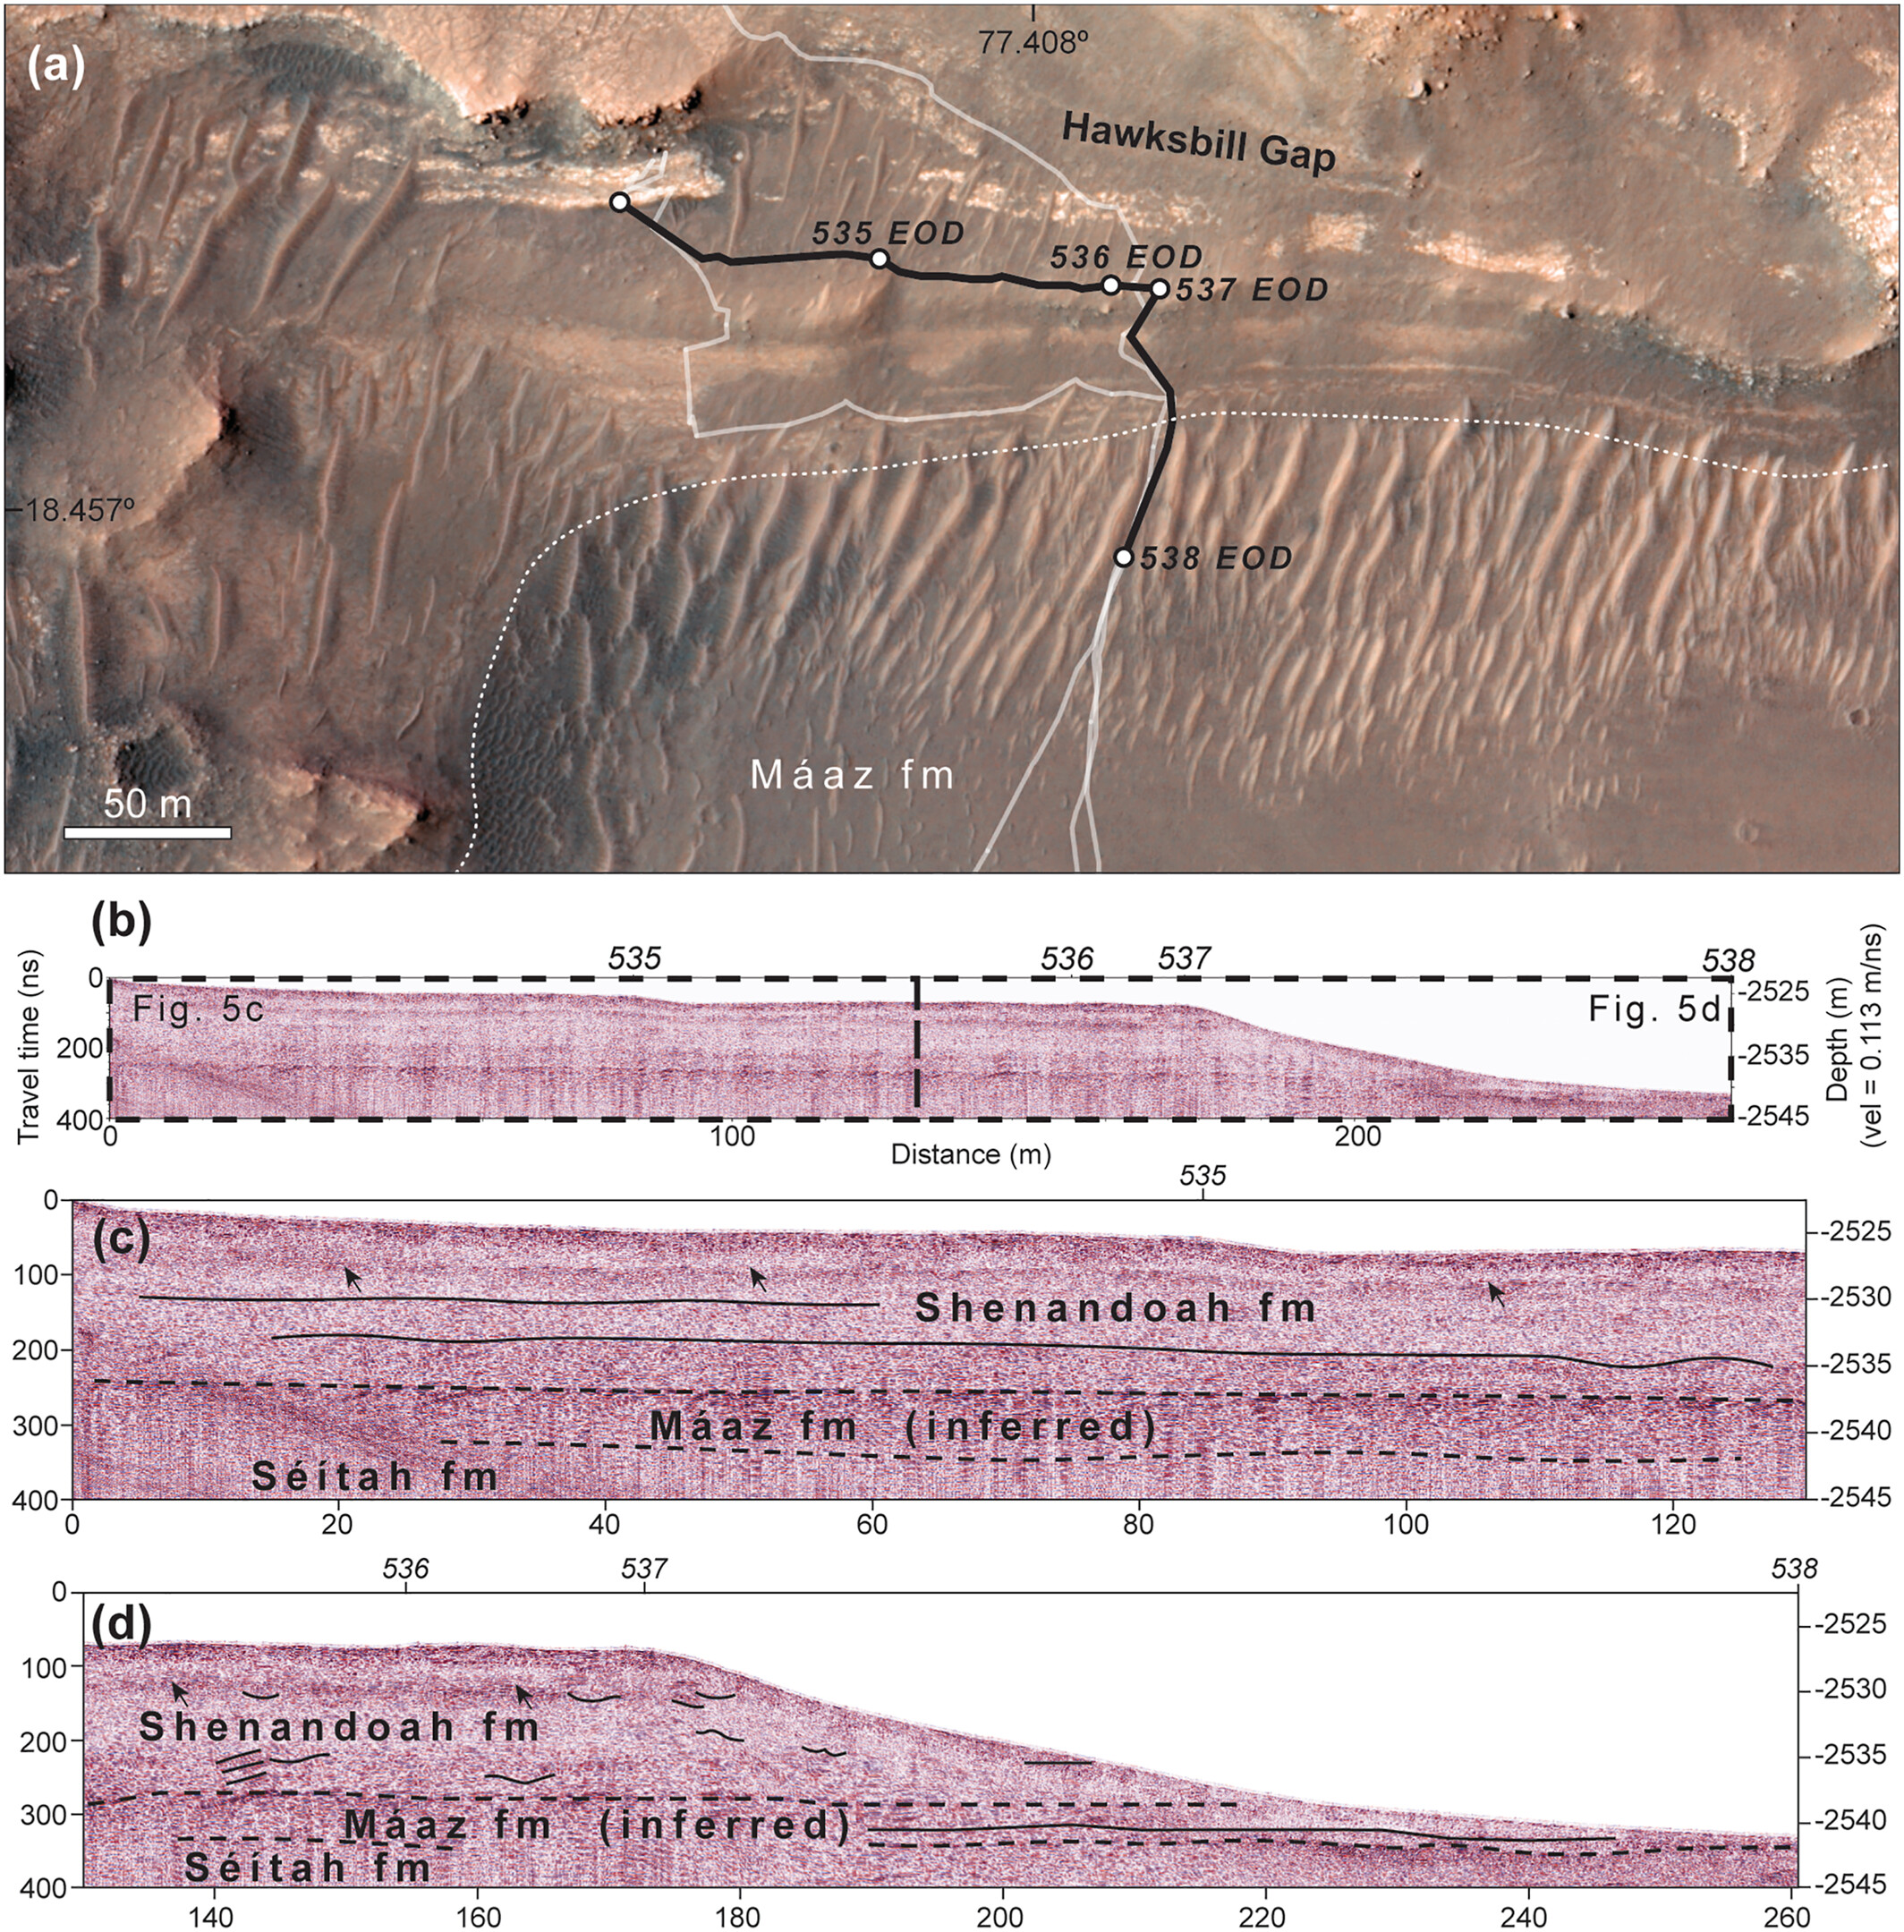
\includegraphics[width=0.9\linewidth]{Figures/0.5RIMFAX/Stack_2024-05.jpg}
    \caption[RIMFAX radargram from sols 535, 536, 537, and 538.]{RIMFAX radargram from sols 535, 536, 537, and 538  \citep{Stack2024}. \textbf{Keywords:} Dipping, horizontal strata, continuous, semi-continuous, low reflectivity, high-reflectivity.}
    \label{fig:Stack24-5}
\end{figure}